% Capitolul 4: Probabilitate
% Statistica piețelor financiare -- Program de licență, Academia de Studii Economice din București
% GENERAT de latex/build_chapter4.py -- modificați generatorul, nu acest fișier.

\newcommand{\coursename}{Statistica piețelor financiare}
\def\sfmlang{ro}
% Preambul comun SFM -- Statistica piețelor financiare / Statistics of Financial Markets (Beamer, 16:9)
% Același design ca MFM. Înainte de % Preambul comun SFM -- Statistica piețelor financiare / Statistics of Financial Markets (Beamer, 16:9)
% Același design ca MFM. Înainte de % Preambul comun SFM -- Statistica piețelor financiare / Statistics of Financial Markets (Beamer, 16:9)
% Același design ca MFM. Înainte de \input{../../latex/preamble} se definește
%   \newcommand{\coursename}{Statistics of Financial Markets}      (EN)
%   \newcommand{\coursename}{Statistica piețelor financiare}       (RO)  și  \def\sfmlang{ro}
% Fișierele .tex se află în EN/Courses, EN/Seminars, RO/Cursuri, RO/Seminarii (două niveluri sub rădăcină).
% Deck-urile sînt generate de latex/build_chapterN.py / build_seminarN.py (vezi latex/sfm_build.py).

\documentclass[9pt, aspectratio=169, t]{beamer}
\providecommand{\coursename}{Statistics of Financial Markets}

% Ensure content fits on slides
\setbeamersize{text margin left=8mm, text margin right=8mm}

%=============================================================================
% THEME AND STYLE CONFIGURATION
%=============================================================================
\usetheme{default}
% Using default theme for clean header/footer control

% Color Palette (matching Redispatch PDF)
\definecolor{MainBlue}{RGB}{26, 58, 110}
\definecolor{AccentBlue}{RGB}{26, 58, 110}
\definecolor{IDAred}{RGB}{205, 0, 0}
\definecolor{DarkGray}{RGB}{51, 51, 51}
\definecolor{MediumGray}{RGB}{128, 128, 128}
\definecolor{LightGray}{RGB}{248, 248, 248}
\definecolor{VeryLightGray}{RGB}{235, 235, 235}
\definecolor{KeynoteGray}{RGB}{218, 218, 218}
\definecolor{SectionGray}{RGB}{120, 120, 120}
\definecolor{FooterGray}{RGB}{100, 100, 100}
\definecolor{Crimson}{RGB}{220, 53, 69}
\definecolor{Forest}{RGB}{46, 125, 50}
\definecolor{Amber}{RGB}{181, 133, 63}
\definecolor{Orange}{RGB}{230, 126, 34}
\definecolor{Purple}{RGB}{142, 68, 173}

% Gradient background (exact Keynote 315° gradient: white to RGB 218,218,218)
\setbeamertemplate{background}{%
    \begin{tikzpicture}[remember picture, overlay]
        \shade[shading=axis, shading angle=315,
        top color=white, bottom color=KeynoteGray]
        (current page.south west) rectangle (current page.north east);
    \end{tikzpicture}%
}
% Fallback solid color for compatibility
\setbeamercolor{background canvas}{bg=}

\setbeamercolor{palette primary}{bg=MainBlue, fg=white}
\setbeamercolor{palette secondary}{bg=MainBlue!85, fg=white}
\setbeamercolor{palette tertiary}{bg=MainBlue!70, fg=white}
\setbeamercolor{structure}{fg=MainBlue}
\setbeamercolor{title}{fg=IDAred}
\setbeamercolor{frametitle}{fg=IDAred, bg=}
\setbeamercolor{block title}{bg=MainBlue, fg=white}
\setbeamercolor{block body}{bg=VeryLightGray, fg=DarkGray}
\setbeamercolor{block title alerted}{bg=Crimson, fg=white}
\setbeamercolor{block body alerted}{bg=Crimson!8, fg=DarkGray}
\setbeamercolor{block title example}{bg=Forest, fg=white}
\setbeamercolor{block body example}{bg=Forest!8, fg=DarkGray}
\setbeamercolor{item}{fg=MainBlue}

% Footer colors (override Madrid theme blue)
\setbeamercolor{author in head/foot}{fg=FooterGray, bg=}
\setbeamercolor{title in head/foot}{fg=FooterGray, bg=}
\setbeamercolor{date in head/foot}{fg=FooterGray, bg=}
\setbeamercolor{section in head/foot}{fg=FooterGray, bg=}
\setbeamercolor{subsection in head/foot}{fg=FooterGray, bg=}

% Bullet styles (apply everywhere including blocks)
\setbeamertemplate{itemize item}{\color{MainBlue}$\boxdot$}
\setbeamertemplate{itemize subitem}{\color{MainBlue}$\blacktriangleright$}
\setbeamertemplate{itemize subsubitem}{\color{MainBlue}\tiny$\bullet$}
\setbeamertemplate{itemize/enumerate body begin}{\normalsize}
\setbeamertemplate{itemize/enumerate subbody begin}{\normalsize}

% Item spacing - compact style
\setlength{\leftmargini}{10pt}       % Level 1: minimal indent
\setlength{\leftmarginii}{10pt}      % Level 2: minimal additional indent
% Compact list spacing (zero extra space before/after lists in blocks)
\makeatletter
\def\@listi{\leftmargin\leftmargini \topsep 0pt \parsep 0pt \itemsep 0pt}
\def\@listii{\leftmargin\leftmarginii \topsep 0pt \parsep 0pt \itemsep 0pt}
\makeatother

\setbeamertemplate{navigation symbols}{}

%=============================================================================
% CUSTOM HEADLINE
%=============================================================================
\setbeamertemplate{headline}{%
    \vskip10pt%
    \hbox to \paperwidth{%
        \hskip0.5cm%
        {\small\color{FooterGray}\renewcommand{\hyperlink}[2]{##2}\insertsectionhead}%
        \hfill%
        \textcolor{FooterGray}{\small\insertframenumber}%
        \hskip0.5cm%
    }%
    \vskip4pt%
    {\color{FooterGray}\hrule height 0.4pt}%
}

%=============================================================================
% CUSTOM FOOTER
%=============================================================================
\usepackage{fontawesome5}

\setbeamertemplate{footline}{%
    {\color{FooterGray}\hrule height 0.4pt}%
    \vskip4pt%
    \hbox to \paperwidth{%
        \hskip0.5cm%
        \textcolor{FooterGray}{\small\coursename}%
        \hfill%
        \raisebox{-0.1em}{%
            \begin{tikzpicture}[x=0.08em, y=0.08em, line width=0.4pt]
                \draw[FooterGray] (0,3) -- (1,4) -- (2,3.5) -- (3,5) -- (4,4) -- (5,6) -- (6,5.5) -- (7,4) -- (8,5) -- (9,7) -- (10,6) -- (11,5) -- (12,6.5) -- (13,8) -- (14,7) -- (15,6) -- (16,7.5) -- (17,9) -- (18,8) -- (19,7) -- (20,8.5) -- (21,10) -- (22,9) -- (23,8) -- (24,9.5);
            \end{tikzpicture}%
        }%
        \hskip0.5cm%
    }%
    \vskip6pt%
}

%=============================================================================
% PACKAGES
%=============================================================================
\usepackage[utf8]{inputenc}
\DeclareUnicodeCharacter{03B1}{\ensuremath{\alpha}}
\usepackage[T1]{fontenc}
\usepackage{amsmath, amssymb, amsthm}
\usepackage{mathtools}
\usepackage{bm}
\usepackage{tikz}
\usetikzlibrary{arrows.meta, positioning, shapes, calc, decorations.pathreplacing, shadings}
\usepackage{booktabs}
\usepackage{multirow}
\usepackage{array}
\usepackage{graphicx}
\usepackage{hyperref}
\usepackage{colortbl}
\usepackage{listings}
\lstset{language=Python, basicstyle=\ttfamily\scriptsize, keywordstyle=\color{MainBlue}\bfseries,
  commentstyle=\color{Forest}, stringstyle=\color{Crimson}, breaklines=true,
  frame=none, backgroundcolor=\color{VeryLightGray}, xleftmargin=2mm}
\hypersetup{colorlinks=true, linkcolor=MainBlue, urlcolor=MainBlue}
\graphicspath{{../../logos/}{../../charts/}{../../photos/}}
\usepackage{xcolor}
\hfuzz=2pt  % Suppress tiny overfull warnings (<2pt)
\vfuzz=2pt  % Suppress tiny vertical overfull warnings (<2pt)

%=============================================================================
% QUANTLET COMMANDS
%   \quantlet{<displayed name>}{<url>}       (generic, compatible with the older SFM decks)
%   \sfmquantlet{Ch_05}{SFM_ch5_garch}       -> https://github.com/danpele/SFM/tree/main/Quantlets/Ch_05/SFM_ch5_garch
%   \qlurl{<folder>} is defined per chapter by the generator (Quantlets/Ch_NN/<folder>)
%=============================================================================
\newcommand{\sfmrepo}{https://github.com/danpele/SFM}
\newcommand{\sfmqlbase}{https://github.com/danpele/SFM/tree/main/Quantlets}
\newcommand{\quantlet}[2]{%
    \hfill\href{#2}{%
        \raisebox{-0.15em}{
\includegraphics[height=0.7em]{ql_logo.png}}%
        \textcolor{MainBlue}{\tiny\ #1}%
    }%
}
\newcommand{\sfmquantlet}[2]{\quantlet{\detokenize{#2}}{\sfmqlbase/#1/#2}}

%=============================================================================
% NOTEBOOKS (Google Colab)
%   \colaburl{notebooks/EN/chapter5_seminar_notebook.ipynb} -> the Colab link of a file in the SFM repo
%   \nb: the chapter notebook (each seminar deck redefines it with \renewcommand)
%=============================================================================
\newcommand{\colaburl}[1]{https://colab.research.google.com/github/danpele/SFM/blob/main/#1}
\newcommand{\nb}{https://colab.research.google.com/github/danpele/SFM/tree/main/notebooks/EN}
\newcommand{\nbname}{notebooks/EN}

%=============================================================================
% SLIDE HELPERS (used by the generators; the same as in MFM)
%=============================================================================
% local font size for list bodies (the preamble forces \normalsize)
\newcommand{\itemsize}[1]{\setbeamertemplate{itemize/enumerate body begin}{#1}\setbeamertemplate{itemize/enumerate subbody begin}{#1}}
\newcommand{\intitle}[1]{{\hypersetup{urlcolor=white}#1}}   % white links inside coloured title bars
\newcommand{\imgcap}[1]{{\scriptsize #1}\\[0.5mm]}          % caption under a photo
\newcommand{\imgcredit}[2]{{\tiny\color{FooterGray}\href{#1}{#2}}}   % image credit: source URL, author/licence
\newcommand{\aiprompt}[1]{{\ttfamily\color{MainBlue}#1}}     % a prompt to an AI assistant

%=============================================================================
% SEMINARS: student version by default; the instructor wrapper *_solutions.tex sets \solutionstrue
%=============================================================================
\makeatletter\@ifundefined{ifsolutions}{\expandafter\newif\csname ifsolutions\endcsname}{}\makeatother
\newcommand{\solonly}[1]{\ifsolutions #1\fi}
\newcommand{\propsub}{\ifsolutions\else\framesubtitle{\ifdefined\sfmlang Rezolvarea se discută la seminar\else Solution discussed in class\fi}\fi}

%=============================================================================
% APPENDIX AND CHAPTER LINKS (latex/appendix_links.py writes the calls; it also re-declares these
% macros before \begin{document}, so the decks compile with or without this preamble block)
%=============================================================================
\providecommand{\sfmapplink}[3]{\hypertarget{#2}{}\hyperlink{#1}{\beamergotobutton{#3}}}
\providecommand{\sfmappback}[2]{\begin{tikzpicture}[remember picture,overlay]\node[anchor=south east] at ([xshift=-3mm,yshift=7mm]current page.south east){\hyperlink{#1}{\beamerreturnbutton{#2}}};\end{tikzpicture}}
\providecommand{\sfmchlink}[2]{\href{#1}{#2}}
\providecommand{\sfmchlinkt}[2]{\href{#1}{\usebeamercolor[fg]{frametitle}#2}}

%=============================================================================
% QUANTINAR COMMAND: link către un curs Quantinar (subiecte avansate)
%=============================================================================
\newcommand{\quantinar}[2]{%
    \href{#2}{%
        \raisebox{-0.15em}{
\includegraphics[height=0.8em]{qr_logo.png}}%
        \textcolor{MainBlue}{\scriptsize\ #1}%
    }%
}

%=============================================================================
% CUSTOM TITLE PAGE
%=============================================================================
\defbeamertemplate*{title page}{hybrid}[1][]
{
    \vspace{0.2cm}
    % Logos row - top header (with clickable links)
    \begin{center}
        \href{https://www.ase.ro}{
\includegraphics[height=1.0cm]{ase_logo.png}}\hspace{0.3cm}%
        \href{https://theida.net}{
\includegraphics[height=1.0cm]{ida_logo.png}}\hspace{0.3cm}%
        \href{https://blockchain-research-center.com}{
\includegraphics[height=1.0cm]{brc_logo.png}}\hspace{0.3cm}%
        \href{https://www.ai4efin.ase.ro}{
\includegraphics[height=1.0cm]{ai4efin_logo.png}}\hspace{0.3cm}%
        \href{https://ipe.ro/new}{
\includegraphics[height=1.0cm]{acad_logo.png}}\hspace{0.3cm}%
        \href{https://www.digital-finance-msca.com}{
\includegraphics[height=1.0cm]{msca_logo.png}}%
    \end{center}

    \vspace{0.6cm}

    % Main title with Q logos on sides (with clickable links)
    \begin{center}
        \begin{minipage}{0.1\textwidth}
            \centering
            \href{https://quantlet.com}{
\includegraphics[height=1.1cm]{ql_logo.png}}
        \end{minipage}%
        \begin{minipage}{0.78\textwidth}
            \centering
            {\LARGE\bfseries\usebeamercolor[fg]{title}\inserttitle}

            \vspace{0.3cm}

            {\usebeamerfont{subtitle}\usebeamercolor[fg]{title}\insertsubtitle}
        \end{minipage}%
        \begin{minipage}{0.1\textwidth}
            \centering
            \href{https://quantinar.com}{
\includegraphics[height=1.1cm]{qr_logo.png}}
        \end{minipage}
    \end{center}

    \vspace{0.6cm}

    % Authors (left aligned)
    \hspace{0.5cm}{\usebeamerfont{author}\insertauthor}

    \vspace{0.3cm}

    % Institute/Affiliations (left aligned)
    \hspace{0.5cm}\begin{minipage}[t]{0.9\textwidth}
        \raggedright\small\insertinstitute
    \end{minipage}
}

%=============================================================================
% THEOREM ENVIRONMENTS
%=============================================================================
\theoremstyle{definition}
\setbeamertemplate{theorems}[numbered]
\ifdefined\sfmlang
\newtheorem{defn}{Definiție}
\newtheorem{thm}{Teoremă}
\newtheorem{prop}{Propoziție}
\newtheorem{rmk}{Observație}
\else
\newtheorem{defn}{Definition}
\newtheorem{thm}{Theorem}
\newtheorem{prop}{Proposition}
\newtheorem{rmk}{Remark}
\fi

%=============================================================================
% CENTRED MINIPAGE (no extra vertical space)
%=============================================================================
\newenvironment{cminipage}[1]{%
    \par\noindent\hfill\begin{minipage}{#1}\ignorespaces
}{%
    \end{minipage}\hfill\null\par
}

%=============================================================================
% CUSTOM COMMANDS
%=============================================================================
\newcommand{\E}{\mathbb{E}}
\newcommand{\Var}{\text{Var}}
\newcommand{\Cov}{\text{Cov}}
\newcommand{\Corr}{\text{Corr}}
\newcommand{\R}{\mathbb{R}}
\newcommand{\N}{\mathbb{N}}
\newcommand{\Z}{\mathbb{Z}}
\newcommand{\B}{\mathbf{B}}
\newcommand{\imark}{\textcolor{MainBlue}{\textbullet}}
\newcommand{\RMSE}{\text{RMSE}}
\newcommand{\MAE}{\text{MAE}}
\newcommand{\MAPE}{\text{MAPE}}

 se definește
%   \newcommand{\coursename}{Statistics of Financial Markets}      (EN)
%   \newcommand{\coursename}{Statistica piețelor financiare}       (RO)  și  \def\sfmlang{ro}
% Fișierele .tex se află în EN/Courses, EN/Seminars, RO/Cursuri, RO/Seminarii (două niveluri sub rădăcină).
% Deck-urile sînt generate de latex/build_chapterN.py / build_seminarN.py (vezi latex/sfm_build.py).

\documentclass[9pt, aspectratio=169, t]{beamer}
\providecommand{\coursename}{Statistics of Financial Markets}

% Ensure content fits on slides
\setbeamersize{text margin left=8mm, text margin right=8mm}

%=============================================================================
% THEME AND STYLE CONFIGURATION
%=============================================================================
\usetheme{default}
% Using default theme for clean header/footer control

% Color Palette (matching Redispatch PDF)
\definecolor{MainBlue}{RGB}{26, 58, 110}
\definecolor{AccentBlue}{RGB}{26, 58, 110}
\definecolor{IDAred}{RGB}{205, 0, 0}
\definecolor{DarkGray}{RGB}{51, 51, 51}
\definecolor{MediumGray}{RGB}{128, 128, 128}
\definecolor{LightGray}{RGB}{248, 248, 248}
\definecolor{VeryLightGray}{RGB}{235, 235, 235}
\definecolor{KeynoteGray}{RGB}{218, 218, 218}
\definecolor{SectionGray}{RGB}{120, 120, 120}
\definecolor{FooterGray}{RGB}{100, 100, 100}
\definecolor{Crimson}{RGB}{220, 53, 69}
\definecolor{Forest}{RGB}{46, 125, 50}
\definecolor{Amber}{RGB}{181, 133, 63}
\definecolor{Orange}{RGB}{230, 126, 34}
\definecolor{Purple}{RGB}{142, 68, 173}

% Gradient background (exact Keynote 315° gradient: white to RGB 218,218,218)
\setbeamertemplate{background}{%
    \begin{tikzpicture}[remember picture, overlay]
        \shade[shading=axis, shading angle=315,
        top color=white, bottom color=KeynoteGray]
        (current page.south west) rectangle (current page.north east);
    \end{tikzpicture}%
}
% Fallback solid color for compatibility
\setbeamercolor{background canvas}{bg=}

\setbeamercolor{palette primary}{bg=MainBlue, fg=white}
\setbeamercolor{palette secondary}{bg=MainBlue!85, fg=white}
\setbeamercolor{palette tertiary}{bg=MainBlue!70, fg=white}
\setbeamercolor{structure}{fg=MainBlue}
\setbeamercolor{title}{fg=IDAred}
\setbeamercolor{frametitle}{fg=IDAred, bg=}
\setbeamercolor{block title}{bg=MainBlue, fg=white}
\setbeamercolor{block body}{bg=VeryLightGray, fg=DarkGray}
\setbeamercolor{block title alerted}{bg=Crimson, fg=white}
\setbeamercolor{block body alerted}{bg=Crimson!8, fg=DarkGray}
\setbeamercolor{block title example}{bg=Forest, fg=white}
\setbeamercolor{block body example}{bg=Forest!8, fg=DarkGray}
\setbeamercolor{item}{fg=MainBlue}

% Footer colors (override Madrid theme blue)
\setbeamercolor{author in head/foot}{fg=FooterGray, bg=}
\setbeamercolor{title in head/foot}{fg=FooterGray, bg=}
\setbeamercolor{date in head/foot}{fg=FooterGray, bg=}
\setbeamercolor{section in head/foot}{fg=FooterGray, bg=}
\setbeamercolor{subsection in head/foot}{fg=FooterGray, bg=}

% Bullet styles (apply everywhere including blocks)
\setbeamertemplate{itemize item}{\color{MainBlue}$\boxdot$}
\setbeamertemplate{itemize subitem}{\color{MainBlue}$\blacktriangleright$}
\setbeamertemplate{itemize subsubitem}{\color{MainBlue}\tiny$\bullet$}
\setbeamertemplate{itemize/enumerate body begin}{\normalsize}
\setbeamertemplate{itemize/enumerate subbody begin}{\normalsize}

% Item spacing - compact style
\setlength{\leftmargini}{10pt}       % Level 1: minimal indent
\setlength{\leftmarginii}{10pt}      % Level 2: minimal additional indent
% Compact list spacing (zero extra space before/after lists in blocks)
\makeatletter
\def\@listi{\leftmargin\leftmargini \topsep 0pt \parsep 0pt \itemsep 0pt}
\def\@listii{\leftmargin\leftmarginii \topsep 0pt \parsep 0pt \itemsep 0pt}
\makeatother

\setbeamertemplate{navigation symbols}{}

%=============================================================================
% CUSTOM HEADLINE
%=============================================================================
\setbeamertemplate{headline}{%
    \vskip10pt%
    \hbox to \paperwidth{%
        \hskip0.5cm%
        {\small\color{FooterGray}\renewcommand{\hyperlink}[2]{##2}\insertsectionhead}%
        \hfill%
        \textcolor{FooterGray}{\small\insertframenumber}%
        \hskip0.5cm%
    }%
    \vskip4pt%
    {\color{FooterGray}\hrule height 0.4pt}%
}

%=============================================================================
% CUSTOM FOOTER
%=============================================================================
\usepackage{fontawesome5}

\setbeamertemplate{footline}{%
    {\color{FooterGray}\hrule height 0.4pt}%
    \vskip4pt%
    \hbox to \paperwidth{%
        \hskip0.5cm%
        \textcolor{FooterGray}{\small\coursename}%
        \hfill%
        \raisebox{-0.1em}{%
            \begin{tikzpicture}[x=0.08em, y=0.08em, line width=0.4pt]
                \draw[FooterGray] (0,3) -- (1,4) -- (2,3.5) -- (3,5) -- (4,4) -- (5,6) -- (6,5.5) -- (7,4) -- (8,5) -- (9,7) -- (10,6) -- (11,5) -- (12,6.5) -- (13,8) -- (14,7) -- (15,6) -- (16,7.5) -- (17,9) -- (18,8) -- (19,7) -- (20,8.5) -- (21,10) -- (22,9) -- (23,8) -- (24,9.5);
            \end{tikzpicture}%
        }%
        \hskip0.5cm%
    }%
    \vskip6pt%
}

%=============================================================================
% PACKAGES
%=============================================================================
\usepackage[utf8]{inputenc}
\DeclareUnicodeCharacter{03B1}{\ensuremath{\alpha}}
\usepackage[T1]{fontenc}
\usepackage{amsmath, amssymb, amsthm}
\usepackage{mathtools}
\usepackage{bm}
\usepackage{tikz}
\usetikzlibrary{arrows.meta, positioning, shapes, calc, decorations.pathreplacing, shadings}
\usepackage{booktabs}
\usepackage{multirow}
\usepackage{array}
\usepackage{graphicx}
\usepackage{hyperref}
\usepackage{colortbl}
\usepackage{listings}
\lstset{language=Python, basicstyle=\ttfamily\scriptsize, keywordstyle=\color{MainBlue}\bfseries,
  commentstyle=\color{Forest}, stringstyle=\color{Crimson}, breaklines=true,
  frame=none, backgroundcolor=\color{VeryLightGray}, xleftmargin=2mm}
\hypersetup{colorlinks=true, linkcolor=MainBlue, urlcolor=MainBlue}
\graphicspath{{../../logos/}{../../charts/}{../../photos/}}
\usepackage{xcolor}
\hfuzz=2pt  % Suppress tiny overfull warnings (<2pt)
\vfuzz=2pt  % Suppress tiny vertical overfull warnings (<2pt)

%=============================================================================
% QUANTLET COMMANDS
%   \quantlet{<displayed name>}{<url>}       (generic, compatible with the older SFM decks)
%   \sfmquantlet{Ch_05}{SFM_ch5_garch}       -> https://github.com/danpele/SFM/tree/main/Quantlets/Ch_05/SFM_ch5_garch
%   \qlurl{<folder>} is defined per chapter by the generator (Quantlets/Ch_NN/<folder>)
%=============================================================================
\newcommand{\sfmrepo}{https://github.com/danpele/SFM}
\newcommand{\sfmqlbase}{https://github.com/danpele/SFM/tree/main/Quantlets}
\newcommand{\quantlet}[2]{%
    \hfill\href{#2}{%
        \raisebox{-0.15em}{
\includegraphics[height=0.7em]{ql_logo.png}}%
        \textcolor{MainBlue}{\tiny\ #1}%
    }%
}
\newcommand{\sfmquantlet}[2]{\quantlet{\detokenize{#2}}{\sfmqlbase/#1/#2}}

%=============================================================================
% NOTEBOOKS (Google Colab)
%   \colaburl{notebooks/EN/chapter5_seminar_notebook.ipynb} -> the Colab link of a file in the SFM repo
%   \nb: the chapter notebook (each seminar deck redefines it with \renewcommand)
%=============================================================================
\newcommand{\colaburl}[1]{https://colab.research.google.com/github/danpele/SFM/blob/main/#1}
\newcommand{\nb}{https://colab.research.google.com/github/danpele/SFM/tree/main/notebooks/EN}
\newcommand{\nbname}{notebooks/EN}

%=============================================================================
% SLIDE HELPERS (used by the generators; the same as in MFM)
%=============================================================================
% local font size for list bodies (the preamble forces \normalsize)
\newcommand{\itemsize}[1]{\setbeamertemplate{itemize/enumerate body begin}{#1}\setbeamertemplate{itemize/enumerate subbody begin}{#1}}
\newcommand{\intitle}[1]{{\hypersetup{urlcolor=white}#1}}   % white links inside coloured title bars
\newcommand{\imgcap}[1]{{\scriptsize #1}\\[0.5mm]}          % caption under a photo
\newcommand{\imgcredit}[2]{{\tiny\color{FooterGray}\href{#1}{#2}}}   % image credit: source URL, author/licence
\newcommand{\aiprompt}[1]{{\ttfamily\color{MainBlue}#1}}     % a prompt to an AI assistant

%=============================================================================
% SEMINARS: student version by default; the instructor wrapper *_solutions.tex sets \solutionstrue
%=============================================================================
\makeatletter\@ifundefined{ifsolutions}{\expandafter\newif\csname ifsolutions\endcsname}{}\makeatother
\newcommand{\solonly}[1]{\ifsolutions #1\fi}
\newcommand{\propsub}{\ifsolutions\else\framesubtitle{\ifdefined\sfmlang Rezolvarea se discută la seminar\else Solution discussed in class\fi}\fi}

%=============================================================================
% APPENDIX AND CHAPTER LINKS (latex/appendix_links.py writes the calls; it also re-declares these
% macros before \begin{document}, so the decks compile with or without this preamble block)
%=============================================================================
\providecommand{\sfmapplink}[3]{\hypertarget{#2}{}\hyperlink{#1}{\beamergotobutton{#3}}}
\providecommand{\sfmappback}[2]{\begin{tikzpicture}[remember picture,overlay]\node[anchor=south east] at ([xshift=-3mm,yshift=7mm]current page.south east){\hyperlink{#1}{\beamerreturnbutton{#2}}};\end{tikzpicture}}
\providecommand{\sfmchlink}[2]{\href{#1}{#2}}
\providecommand{\sfmchlinkt}[2]{\href{#1}{\usebeamercolor[fg]{frametitle}#2}}

%=============================================================================
% QUANTINAR COMMAND: link către un curs Quantinar (subiecte avansate)
%=============================================================================
\newcommand{\quantinar}[2]{%
    \href{#2}{%
        \raisebox{-0.15em}{
\includegraphics[height=0.8em]{qr_logo.png}}%
        \textcolor{MainBlue}{\scriptsize\ #1}%
    }%
}

%=============================================================================
% CUSTOM TITLE PAGE
%=============================================================================
\defbeamertemplate*{title page}{hybrid}[1][]
{
    \vspace{0.2cm}
    % Logos row - top header (with clickable links)
    \begin{center}
        \href{https://www.ase.ro}{
\includegraphics[height=1.0cm]{ase_logo.png}}\hspace{0.3cm}%
        \href{https://theida.net}{
\includegraphics[height=1.0cm]{ida_logo.png}}\hspace{0.3cm}%
        \href{https://blockchain-research-center.com}{
\includegraphics[height=1.0cm]{brc_logo.png}}\hspace{0.3cm}%
        \href{https://www.ai4efin.ase.ro}{
\includegraphics[height=1.0cm]{ai4efin_logo.png}}\hspace{0.3cm}%
        \href{https://ipe.ro/new}{
\includegraphics[height=1.0cm]{acad_logo.png}}\hspace{0.3cm}%
        \href{https://www.digital-finance-msca.com}{
\includegraphics[height=1.0cm]{msca_logo.png}}%
    \end{center}

    \vspace{0.6cm}

    % Main title with Q logos on sides (with clickable links)
    \begin{center}
        \begin{minipage}{0.1\textwidth}
            \centering
            \href{https://quantlet.com}{
\includegraphics[height=1.1cm]{ql_logo.png}}
        \end{minipage}%
        \begin{minipage}{0.78\textwidth}
            \centering
            {\LARGE\bfseries\usebeamercolor[fg]{title}\inserttitle}

            \vspace{0.3cm}

            {\usebeamerfont{subtitle}\usebeamercolor[fg]{title}\insertsubtitle}
        \end{minipage}%
        \begin{minipage}{0.1\textwidth}
            \centering
            \href{https://quantinar.com}{
\includegraphics[height=1.1cm]{qr_logo.png}}
        \end{minipage}
    \end{center}

    \vspace{0.6cm}

    % Authors (left aligned)
    \hspace{0.5cm}{\usebeamerfont{author}\insertauthor}

    \vspace{0.3cm}

    % Institute/Affiliations (left aligned)
    \hspace{0.5cm}\begin{minipage}[t]{0.9\textwidth}
        \raggedright\small\insertinstitute
    \end{minipage}
}

%=============================================================================
% THEOREM ENVIRONMENTS
%=============================================================================
\theoremstyle{definition}
\setbeamertemplate{theorems}[numbered]
\ifdefined\sfmlang
\newtheorem{defn}{Definiție}
\newtheorem{thm}{Teoremă}
\newtheorem{prop}{Propoziție}
\newtheorem{rmk}{Observație}
\else
\newtheorem{defn}{Definition}
\newtheorem{thm}{Theorem}
\newtheorem{prop}{Proposition}
\newtheorem{rmk}{Remark}
\fi

%=============================================================================
% CENTRED MINIPAGE (no extra vertical space)
%=============================================================================
\newenvironment{cminipage}[1]{%
    \par\noindent\hfill\begin{minipage}{#1}\ignorespaces
}{%
    \end{minipage}\hfill\null\par
}

%=============================================================================
% CUSTOM COMMANDS
%=============================================================================
\newcommand{\E}{\mathbb{E}}
\newcommand{\Var}{\text{Var}}
\newcommand{\Cov}{\text{Cov}}
\newcommand{\Corr}{\text{Corr}}
\newcommand{\R}{\mathbb{R}}
\newcommand{\N}{\mathbb{N}}
\newcommand{\Z}{\mathbb{Z}}
\newcommand{\B}{\mathbf{B}}
\newcommand{\imark}{\textcolor{MainBlue}{\textbullet}}
\newcommand{\RMSE}{\text{RMSE}}
\newcommand{\MAE}{\text{MAE}}
\newcommand{\MAPE}{\text{MAPE}}

 se definește
%   \newcommand{\coursename}{Statistics of Financial Markets}      (EN)
%   \newcommand{\coursename}{Statistica piețelor financiare}       (RO)  și  \def\sfmlang{ro}
% Fișierele .tex se află în EN/Courses, EN/Seminars, RO/Cursuri, RO/Seminarii (două niveluri sub rădăcină).
% Deck-urile sînt generate de latex/build_chapterN.py / build_seminarN.py (vezi latex/sfm_build.py).

\documentclass[9pt, aspectratio=169, t]{beamer}
\providecommand{\coursename}{Statistics of Financial Markets}

% Ensure content fits on slides
\setbeamersize{text margin left=8mm, text margin right=8mm}

%=============================================================================
% THEME AND STYLE CONFIGURATION
%=============================================================================
\usetheme{default}
% Using default theme for clean header/footer control

% Color Palette (matching Redispatch PDF)
\definecolor{MainBlue}{RGB}{26, 58, 110}
\definecolor{AccentBlue}{RGB}{26, 58, 110}
\definecolor{IDAred}{RGB}{205, 0, 0}
\definecolor{DarkGray}{RGB}{51, 51, 51}
\definecolor{MediumGray}{RGB}{128, 128, 128}
\definecolor{LightGray}{RGB}{248, 248, 248}
\definecolor{VeryLightGray}{RGB}{235, 235, 235}
\definecolor{KeynoteGray}{RGB}{218, 218, 218}
\definecolor{SectionGray}{RGB}{120, 120, 120}
\definecolor{FooterGray}{RGB}{100, 100, 100}
\definecolor{Crimson}{RGB}{220, 53, 69}
\definecolor{Forest}{RGB}{46, 125, 50}
\definecolor{Amber}{RGB}{181, 133, 63}
\definecolor{Orange}{RGB}{230, 126, 34}
\definecolor{Purple}{RGB}{142, 68, 173}

% Gradient background (exact Keynote 315° gradient: white to RGB 218,218,218)
\setbeamertemplate{background}{%
    \begin{tikzpicture}[remember picture, overlay]
        \shade[shading=axis, shading angle=315,
        top color=white, bottom color=KeynoteGray]
        (current page.south west) rectangle (current page.north east);
    \end{tikzpicture}%
}
% Fallback solid color for compatibility
\setbeamercolor{background canvas}{bg=}

\setbeamercolor{palette primary}{bg=MainBlue, fg=white}
\setbeamercolor{palette secondary}{bg=MainBlue!85, fg=white}
\setbeamercolor{palette tertiary}{bg=MainBlue!70, fg=white}
\setbeamercolor{structure}{fg=MainBlue}
\setbeamercolor{title}{fg=IDAred}
\setbeamercolor{frametitle}{fg=IDAred, bg=}
\setbeamercolor{block title}{bg=MainBlue, fg=white}
\setbeamercolor{block body}{bg=VeryLightGray, fg=DarkGray}
\setbeamercolor{block title alerted}{bg=Crimson, fg=white}
\setbeamercolor{block body alerted}{bg=Crimson!8, fg=DarkGray}
\setbeamercolor{block title example}{bg=Forest, fg=white}
\setbeamercolor{block body example}{bg=Forest!8, fg=DarkGray}
\setbeamercolor{item}{fg=MainBlue}

% Footer colors (override Madrid theme blue)
\setbeamercolor{author in head/foot}{fg=FooterGray, bg=}
\setbeamercolor{title in head/foot}{fg=FooterGray, bg=}
\setbeamercolor{date in head/foot}{fg=FooterGray, bg=}
\setbeamercolor{section in head/foot}{fg=FooterGray, bg=}
\setbeamercolor{subsection in head/foot}{fg=FooterGray, bg=}

% Bullet styles (apply everywhere including blocks)
\setbeamertemplate{itemize item}{\color{MainBlue}$\boxdot$}
\setbeamertemplate{itemize subitem}{\color{MainBlue}$\blacktriangleright$}
\setbeamertemplate{itemize subsubitem}{\color{MainBlue}\tiny$\bullet$}
\setbeamertemplate{itemize/enumerate body begin}{\normalsize}
\setbeamertemplate{itemize/enumerate subbody begin}{\normalsize}

% Item spacing - compact style
\setlength{\leftmargini}{10pt}       % Level 1: minimal indent
\setlength{\leftmarginii}{10pt}      % Level 2: minimal additional indent
% Compact list spacing (zero extra space before/after lists in blocks)
\makeatletter
\def\@listi{\leftmargin\leftmargini \topsep 0pt \parsep 0pt \itemsep 0pt}
\def\@listii{\leftmargin\leftmarginii \topsep 0pt \parsep 0pt \itemsep 0pt}
\makeatother

\setbeamertemplate{navigation symbols}{}

%=============================================================================
% CUSTOM HEADLINE
%=============================================================================
\setbeamertemplate{headline}{%
    \vskip10pt%
    \hbox to \paperwidth{%
        \hskip0.5cm%
        {\small\color{FooterGray}\renewcommand{\hyperlink}[2]{##2}\insertsectionhead}%
        \hfill%
        \textcolor{FooterGray}{\small\insertframenumber}%
        \hskip0.5cm%
    }%
    \vskip4pt%
    {\color{FooterGray}\hrule height 0.4pt}%
}

%=============================================================================
% CUSTOM FOOTER
%=============================================================================
\usepackage{fontawesome5}

\setbeamertemplate{footline}{%
    {\color{FooterGray}\hrule height 0.4pt}%
    \vskip4pt%
    \hbox to \paperwidth{%
        \hskip0.5cm%
        \textcolor{FooterGray}{\small\coursename}%
        \hfill%
        \raisebox{-0.1em}{%
            \begin{tikzpicture}[x=0.08em, y=0.08em, line width=0.4pt]
                \draw[FooterGray] (0,3) -- (1,4) -- (2,3.5) -- (3,5) -- (4,4) -- (5,6) -- (6,5.5) -- (7,4) -- (8,5) -- (9,7) -- (10,6) -- (11,5) -- (12,6.5) -- (13,8) -- (14,7) -- (15,6) -- (16,7.5) -- (17,9) -- (18,8) -- (19,7) -- (20,8.5) -- (21,10) -- (22,9) -- (23,8) -- (24,9.5);
            \end{tikzpicture}%
        }%
        \hskip0.5cm%
    }%
    \vskip6pt%
}

%=============================================================================
% PACKAGES
%=============================================================================
\usepackage[utf8]{inputenc}
\DeclareUnicodeCharacter{03B1}{\ensuremath{\alpha}}
\usepackage[T1]{fontenc}
\usepackage{amsmath, amssymb, amsthm}
\usepackage{mathtools}
\usepackage{bm}
\usepackage{tikz}
\usetikzlibrary{arrows.meta, positioning, shapes, calc, decorations.pathreplacing, shadings}
\usepackage{booktabs}
\usepackage{multirow}
\usepackage{array}
\usepackage{graphicx}
\usepackage{hyperref}
\usepackage{colortbl}
\usepackage{listings}
\lstset{language=Python, basicstyle=\ttfamily\scriptsize, keywordstyle=\color{MainBlue}\bfseries,
  commentstyle=\color{Forest}, stringstyle=\color{Crimson}, breaklines=true,
  frame=none, backgroundcolor=\color{VeryLightGray}, xleftmargin=2mm}
\hypersetup{colorlinks=true, linkcolor=MainBlue, urlcolor=MainBlue}
\graphicspath{{../../logos/}{../../charts/}{../../photos/}}
\usepackage{xcolor}
\hfuzz=2pt  % Suppress tiny overfull warnings (<2pt)
\vfuzz=2pt  % Suppress tiny vertical overfull warnings (<2pt)

%=============================================================================
% QUANTLET COMMANDS
%   \quantlet{<displayed name>}{<url>}       (generic, compatible with the older SFM decks)
%   \sfmquantlet{Ch_05}{SFM_ch5_garch}       -> https://github.com/danpele/SFM/tree/main/Quantlets/Ch_05/SFM_ch5_garch
%   \qlurl{<folder>} is defined per chapter by the generator (Quantlets/Ch_NN/<folder>)
%=============================================================================
\newcommand{\sfmrepo}{https://github.com/danpele/SFM}
\newcommand{\sfmqlbase}{https://github.com/danpele/SFM/tree/main/Quantlets}
\newcommand{\quantlet}[2]{%
    \hfill\href{#2}{%
        \raisebox{-0.15em}{
\includegraphics[height=0.7em]{ql_logo.png}}%
        \textcolor{MainBlue}{\tiny\ #1}%
    }%
}
\newcommand{\sfmquantlet}[2]{\quantlet{\detokenize{#2}}{\sfmqlbase/#1/#2}}

%=============================================================================
% NOTEBOOKS (Google Colab)
%   \colaburl{notebooks/EN/chapter5_seminar_notebook.ipynb} -> the Colab link of a file in the SFM repo
%   \nb: the chapter notebook (each seminar deck redefines it with \renewcommand)
%=============================================================================
\newcommand{\colaburl}[1]{https://colab.research.google.com/github/danpele/SFM/blob/main/#1}
\newcommand{\nb}{https://colab.research.google.com/github/danpele/SFM/tree/main/notebooks/EN}
\newcommand{\nbname}{notebooks/EN}

%=============================================================================
% SLIDE HELPERS (used by the generators; the same as in MFM)
%=============================================================================
% local font size for list bodies (the preamble forces \normalsize)
\newcommand{\itemsize}[1]{\setbeamertemplate{itemize/enumerate body begin}{#1}\setbeamertemplate{itemize/enumerate subbody begin}{#1}}
\newcommand{\intitle}[1]{{\hypersetup{urlcolor=white}#1}}   % white links inside coloured title bars
\newcommand{\imgcap}[1]{{\scriptsize #1}\\[0.5mm]}          % caption under a photo
\newcommand{\imgcredit}[2]{{\tiny\color{FooterGray}\href{#1}{#2}}}   % image credit: source URL, author/licence
\newcommand{\aiprompt}[1]{{\ttfamily\color{MainBlue}#1}}     % a prompt to an AI assistant

%=============================================================================
% SEMINARS: student version by default; the instructor wrapper *_solutions.tex sets \solutionstrue
%=============================================================================
\makeatletter\@ifundefined{ifsolutions}{\expandafter\newif\csname ifsolutions\endcsname}{}\makeatother
\newcommand{\solonly}[1]{\ifsolutions #1\fi}
\newcommand{\propsub}{\ifsolutions\else\framesubtitle{\ifdefined\sfmlang Rezolvarea se discută la seminar\else Solution discussed in class\fi}\fi}

%=============================================================================
% APPENDIX AND CHAPTER LINKS (latex/appendix_links.py writes the calls; it also re-declares these
% macros before \begin{document}, so the decks compile with or without this preamble block)
%=============================================================================
\providecommand{\sfmapplink}[3]{\hypertarget{#2}{}\hyperlink{#1}{\beamergotobutton{#3}}}
\providecommand{\sfmappback}[2]{\begin{tikzpicture}[remember picture,overlay]\node[anchor=south east] at ([xshift=-3mm,yshift=7mm]current page.south east){\hyperlink{#1}{\beamerreturnbutton{#2}}};\end{tikzpicture}}
\providecommand{\sfmchlink}[2]{\href{#1}{#2}}
\providecommand{\sfmchlinkt}[2]{\href{#1}{\usebeamercolor[fg]{frametitle}#2}}

%=============================================================================
% QUANTINAR COMMAND: link către un curs Quantinar (subiecte avansate)
%=============================================================================
\newcommand{\quantinar}[2]{%
    \href{#2}{%
        \raisebox{-0.15em}{
\includegraphics[height=0.8em]{qr_logo.png}}%
        \textcolor{MainBlue}{\scriptsize\ #1}%
    }%
}

%=============================================================================
% CUSTOM TITLE PAGE
%=============================================================================
\defbeamertemplate*{title page}{hybrid}[1][]
{
    \vspace{0.2cm}
    % Logos row - top header (with clickable links)
    \begin{center}
        \href{https://www.ase.ro}{
\includegraphics[height=1.0cm]{ase_logo.png}}\hspace{0.3cm}%
        \href{https://theida.net}{
\includegraphics[height=1.0cm]{ida_logo.png}}\hspace{0.3cm}%
        \href{https://blockchain-research-center.com}{
\includegraphics[height=1.0cm]{brc_logo.png}}\hspace{0.3cm}%
        \href{https://www.ai4efin.ase.ro}{
\includegraphics[height=1.0cm]{ai4efin_logo.png}}\hspace{0.3cm}%
        \href{https://ipe.ro/new}{
\includegraphics[height=1.0cm]{acad_logo.png}}\hspace{0.3cm}%
        \href{https://www.digital-finance-msca.com}{
\includegraphics[height=1.0cm]{msca_logo.png}}%
    \end{center}

    \vspace{0.6cm}

    % Main title with Q logos on sides (with clickable links)
    \begin{center}
        \begin{minipage}{0.1\textwidth}
            \centering
            \href{https://quantlet.com}{
\includegraphics[height=1.1cm]{ql_logo.png}}
        \end{minipage}%
        \begin{minipage}{0.78\textwidth}
            \centering
            {\LARGE\bfseries\usebeamercolor[fg]{title}\inserttitle}

            \vspace{0.3cm}

            {\usebeamerfont{subtitle}\usebeamercolor[fg]{title}\insertsubtitle}
        \end{minipage}%
        \begin{minipage}{0.1\textwidth}
            \centering
            \href{https://quantinar.com}{
\includegraphics[height=1.1cm]{qr_logo.png}}
        \end{minipage}
    \end{center}

    \vspace{0.6cm}

    % Authors (left aligned)
    \hspace{0.5cm}{\usebeamerfont{author}\insertauthor}

    \vspace{0.3cm}

    % Institute/Affiliations (left aligned)
    \hspace{0.5cm}\begin{minipage}[t]{0.9\textwidth}
        \raggedright\small\insertinstitute
    \end{minipage}
}

%=============================================================================
% THEOREM ENVIRONMENTS
%=============================================================================
\theoremstyle{definition}
\setbeamertemplate{theorems}[numbered]
\ifdefined\sfmlang
\newtheorem{defn}{Definiție}
\newtheorem{thm}{Teoremă}
\newtheorem{prop}{Propoziție}
\newtheorem{rmk}{Observație}
\else
\newtheorem{defn}{Definition}
\newtheorem{thm}{Theorem}
\newtheorem{prop}{Proposition}
\newtheorem{rmk}{Remark}
\fi

%=============================================================================
% CENTRED MINIPAGE (no extra vertical space)
%=============================================================================
\newenvironment{cminipage}[1]{%
    \par\noindent\hfill\begin{minipage}{#1}\ignorespaces
}{%
    \end{minipage}\hfill\null\par
}

%=============================================================================
% CUSTOM COMMANDS
%=============================================================================
\newcommand{\E}{\mathbb{E}}
\newcommand{\Var}{\text{Var}}
\newcommand{\Cov}{\text{Cov}}
\newcommand{\Corr}{\text{Corr}}
\newcommand{\R}{\mathbb{R}}
\newcommand{\N}{\mathbb{N}}
\newcommand{\Z}{\mathbb{Z}}
\newcommand{\B}{\mathbf{B}}
\newcommand{\imark}{\textcolor{MainBlue}{\textbullet}}
\newcommand{\RMSE}{\text{RMSE}}
\newcommand{\MAE}{\text{MAE}}
\newcommand{\MAPE}{\text{MAPE}}



\newcommand{\qlurl}[1]{https://github.com/danpele/SFM/tree/main/Quantlets/Ch_04/#1}

% Clickable citations (DOIs verified via Crossref)

\newcommand{\refFHH}{\href{https://doi.org/10.1007/978-3-030-13751-9}{Franke, Härdle \& Hafner (2019)}}
\newcommand{\refFHHex}{\href{https://doi.org/10.1007/978-3-642-33929-5}{Borak, Härdle \& López-Cabrera (2013)}}
\newcommand{\refKolmogorov}{\href{https://doi.org/10.1007/978-3-642-49888-6}{Kolmogoroff (1933)}}
\newcommand{\refBachelier}{\href{https://doi.org/10.24033/asens.476}{Bachelier (1900)}}
\newcommand{\refEinstein}{\href{https://doi.org/10.1002/andp.19053220806}{Einstein (1905)}}
\newcommand{\refWiener}{\href{https://doi.org/10.1002/sapm192321131}{Wiener (1923)}}
\newcommand{\refOsborne}{\href{https://doi.org/10.1287/opre.7.2.145}{Osborne (1959)}}
\newcommand{\refBS}{\href{https://doi.org/10.1086/260062}{Black \& Scholes (1973)}}
\newcommand{\refCRR}{\href{https://doi.org/10.1016/0304-405X(79)90015-1}{Cox, Ross \& Rubinstein (1979)}}
\newcommand{\refMU}{\href{https://doi.org/10.1080/01621459.1949.10483310}{Metropolis \& Ulam (1949)}}
\newcommand{\refMarsaglia}{\href{https://doi.org/10.1073/pnas.61.1.25}{Marsaglia (1968)}}
\newcommand{\refMT}{\href{https://doi.org/10.1145/272991.272995}{Matsumoto \& Nishimura (1998)}}
\newcommand{\refGlasserman}{\href{https://doi.org/10.1007/978-0-387-21617-1}{Glasserman (2003)}}
\newcommand{\refEngle}{\href{https://doi.org/10.2307/1912773}{Engle (1982)}}
\newcommand{\refBollerslev}{\href{https://doi.org/10.1016/0304-4076(86)90063-1}{Bollerslev (1986)}}
\newcommand{\refFama}{\href{https://doi.org/10.2307/2325486}{Fama (1970)}}
\newcommand{\refCont}{\href{https://doi.org/10.1080/713665670}{Cont (2001)}}
\newcommand{\refPeleCrypto}{\href{https://doi.org/10.1080/1351847X.2021.1960403}{Pele et al.\ (2023)}}
\newcommand{\refWang}{\href{https://doi.org/10.1038/s41586-023-06221-2}{Wang et al.\ (2023)}}

\title[Statistica piețelor financiare]{Statistica piețelor financiare}
\subtitle{Capitolul 4: Probabilitate}
\author[D.T. Pele]{Daniel Traian PELE}
\institute{Academia de Studii Economice din București\\
IDA Institute Digital Assets\\
Blockchain Research Center\\
AI4EFin Artificial Intelligence for Energy Finance\\
Academia Română, Institutul de Prognoză Economică\\
MSCA Digital Finance}
\date{}

%=============================================================================
\providecommand{\sfmapplink}[3]{\hypertarget{#2}{}\hyperlink{#1}{\beamergotobutton{#3}}}  % APPLINKS-MACROS
\providecommand{\sfmappback}[2]{\begin{tikzpicture}[remember picture,overlay]\node[anchor=south east] at ([xshift=-3mm,yshift=7mm]current page.south east){\hyperlink{#1}{\beamerreturnbutton{#2}}};\end{tikzpicture}}  % APPLINKS-MACROS
\providecommand{\sfmchlink}[2]{\href{#1}{#2}}  % APPLINKS-MACROS
\providecommand{\sfmchlinkt}[2]{\href{#1}{\usebeamercolor[fg]{frametitle}#2}}  % APPLINKS-MACROS
\begin{document}
%=============================================================================

{
\setbeamertemplate{headline}{}
\setbeamertemplate{footline}{}
\begin{frame}[noframenumbering]
    \titlepage
\end{frame}
}
% BEGIN-ACRONYMS (generat de latex/acronyms.py; nu editati manual)
\begin{frame}{Acronime folosite în acest material}
\setbeamertemplate{itemize/enumerate body begin}{\footnotesize}
\begin{columns}[T]
\begin{column}{0.49\textwidth}
\begin{itemize}\setlength{\itemsep}{0pt}
    \item \textbf{AI}: Artificial Intelligence (inteligență artificială)
    \item \textbf{AR}: AutoRegressive (model) — model autoregresiv
    \item \textbf{ARCH}: AutoRegressive Conditional Heteroskedasticity (heteroscedasticitate condiționată autoregresivă)
    \item \textbf{BET}: Bucharest Exchange Trading (index) — indicele de referință al Bursei de Valori București
    \item \textbf{CDF}: Cumulative Distribution Function (funcția de repartiție)
    \item \textbf{CLT}: Central Limit Theorem (teorema limită centrală)
    \item \textbf{CRR}: Cox–Ross–Rubinstein (binomial model) — modelul binomial Cox–Ross–Rubinstein
    \item \textbf{GARCH}: Generalised AutoRegressive Conditional Heteroskedasticity (heteroscedasticitate condiționată autoregresivă generalizată)
    \item \textbf{GBM}: Geometric Brownian Motion (mișcarea browniană geometrică)
\end{itemize}
\end{column}
\begin{column}{0.49\textwidth}
\begin{itemize}\setlength{\itemsep}{0pt}
    \item \textbf{IBM}: International Business Machines (company) — compania International Business Machines
    \item \textbf{LCG}: Linear Congruential Generator (generator congruențial liniar)
    \item \textbf{LLN}: Law of Large Numbers (legea numerelor mari)
    \item \textbf{PCG64}: Permuted Congruential Generator, 64-bit (NumPy default) — generatorul congruențial permutat pe 64 de biți (implicit în NumPy)
    \item \textbf{PMF}: Probability Mass Function (funcția de masă de probabilitate)
    \item \textbf{RANDU}: RANDU (IBM random number generator of the 1960s) — generatorul de numere aleatoare RANDU al IBM, anii 1960
    \item \textbf{SFE}: Statistics of Financial Markets, Exercises (Quantlet collection of the textbook) — colecția de Quantlet-uri a manualului Statistics of Financial Markets
\end{itemize}
\end{column}
\end{columns}
\end{frame}
% END-ACRONYMS

\begin{frame}{Întrebarea de azi și traseul}
\itemsize{\small}
\begin{itemize}
    \item \textbf{Întrebarea}: de ce instrumente de probabilitate avem nevoie pentru a descrie randamentele și pentru a simula prețuri?
    \begin{itemize}
        \item toate capitolele următoare (cozi, volatilitate, VaR, eficiență) se sprijină pe ele
    \end{itemize}
    \item \textbf{Traseul} capitolului
    \begin{itemize}
        \item variabile aleatoare, distribuții, speranță matematică, varianță, covarianță
        \item independență și necorelare, speranța condiționată și varianța condiționată
        \item numere aleatoare și Monte Carlo; modelul binomial
        \item mers aleator, martingal, zgomot alb, AR(1); procesul Wiener și GBM
    \end{itemize}
    \item Date reale, 2000--2026: S\&P 500, DAX, BET și Bitcoin (din 2014)
\end{itemize}
\end{frame}

\begin{frame}{Rezultatele învățării}
\itemsize{\small}
\begin{itemize}
    \item Calculați speranțe matematice, varianțe, covarianțe și corelații, precum și volatilitatea unui portofoliu
    \item Explicați de ce randamente necorelate pot fi totuși dependente și măsurați acest lucru
    \item Folosiți speranța condiționată și varianța condiționată, elementele de bază ale modelelor GARCH
    \item Generați numere aleatoare prin metoda transformării inverse și estimați o probabilitate prin Monte Carlo, cu eroarea ei standard
    \item Definiți mersul aleator, martingalul, zgomotul alb, procesul Wiener și GBM și simulați-le
\end{itemize}
\end{frame}

\begin{frame}{Bibliografie și instrumente}
\itemsize{\small}
\begin{itemize}
    \item Manual: \refFHH, \textit{Statistics of Financial Markets}, ed. a 5-a, cap.~3 (secț.~3.1--3.5) și cap.~4 (procese stochastice în timp discret)
    \begin{itemize}
        \item exerciții rezolvate: \refFHHex, cap.~3--4
    \end{itemize}
    \item Metode Monte Carlo în finanțe: \refGlasserman
    \item Quantlet-urile Python ale capitolului: \href{https://github.com/danpele/SFM/tree/main/Quantlets/Ch_04}{Quantlets/Ch\_04}
    \begin{itemize}
        \item portate din Quantlet-urile SFE ale manualului (SFErandu, SFErangen1, SFErangen2, SFEBinomp, SFEWienerProcess, SFEsimGBM)
        \item fiecare grafic din aceste slide-uri are legătură către Quantlet-ul care îl desenează
    \end{itemize}
    \item Notebook-ul cursului: \href{\colaburl{notebooks/EN/chapter4_lecture_notebook.ipynb}}{deschideți în Google Colab}
    \item Curs video: \quantinar{Statistics of Financial Markets}{https://quantinar.com/course/103/statistics-of-financial-markets}
\end{itemize}
\end{frame}


%=============================================================================
\section{De la jocuri de noroc la axiome}
%=============================================================================

\begin{frame}{1654: problema punctelor}
\itemsize{\small}
\begin{columns}[T]
\begin{column}{0.60\textwidth}
\begin{itemize}
    \item Doi jucători opresc un joc echitabil înainte de final: cum se împarte miza?
    \item Blaise Pascal și Pierre de Fermat au rezolvat-o prin scrisori (1654): împărțim după probabilitatea de a cîștiga, nu după scor
    \item Exemplu: lui A îi mai trebuie 1 victorie, lui B 2; cel mult încă două runde
    \begin{itemize}
        \item B cîștigă doar dacă cîștigă ambele runde: probabilitatea $1/4$
        \item A trebuie să primească 75\% din miză: cîștigul lui \textbf{așteptat}
    \end{itemize}
    \item Aceeași idee stă azi la baza evaluării derivatelor: prețul corect este o plată așteptată
\end{itemize}
\end{column}
\begin{column}{0.36\textwidth}
\centering
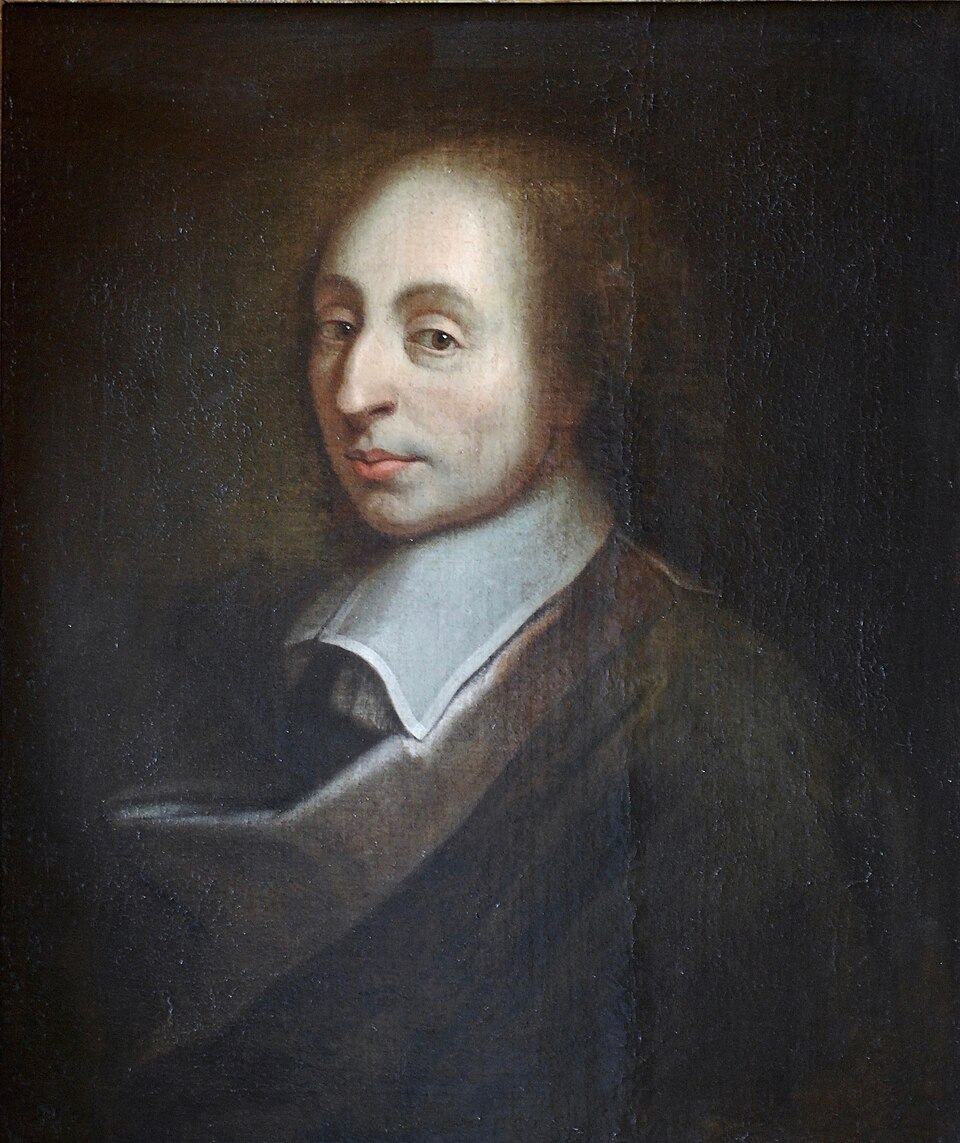
\includegraphics[height=0.55\textheight]{ch4_pascal.jpg}\\[1mm]
\imgcap{Blaise Pascal (1623--1662)}
\imgcredit{https://commons.wikimedia.org/wiki/File:Blaise_Pascal_Versailles.JPG}{Portret: autor necunoscut, după François II Quesnel (c. 1690); domeniu public; Wikimedia Commons}
\end{column}
\end{columns}
\end{frame}

\begin{frame}{Axiomele lui Kolmogorov (1933)}
\itemsize{\footnotesize}
\begin{columns}[T]
\begin{column}{0.62\textwidth}
\begin{itemize}
    \item Un \textbf{spațiu de probabilitate} $(\Omega, \mathcal{F}, P)$ \refKolmogorov
    \begin{itemize}
        \item $\Omega$: toate rezultatele posibile (toate traiectoriile posibile ale pieței de mîine)
        \item $\mathcal{F}$: evenimentele cărora le putem atribui o probabilitate (o $\sigma$-algebră)
        \item $P$: o funcție de la evenimente la $[0, 1]$
    \end{itemize}
    \item Axiomele, pentru orice eveniment $A \in \mathcal{F}$
    \begin{itemize}
        \item $P(A) \ge 0$: nicio probabilitate nu este negativă
        \item $P(\Omega) = 1$: unul dintre rezultate are loc sigur
        \item $P(\cup_i A_i) = \sum_i P(A_i)$ pentru $A_1, A_2, \dots$ disjuncte (oricare două nu pot avea loc simultan): probabilitatea ca unul dintre ele să aibă loc este suma probabilităților
    \end{itemize}
    \item Tot restul (speranță, independență, procese) se construiește pe aceste trei reguli
\end{itemize}
\end{column}
\begin{column}{0.34\textwidth}
\centering
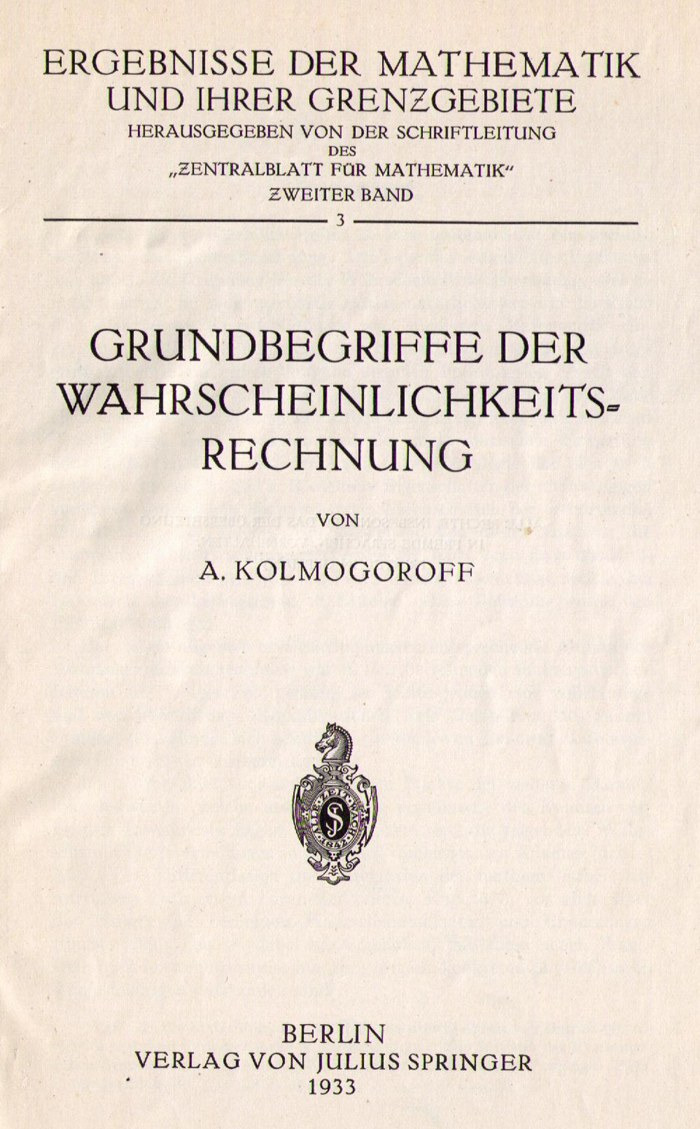
\includegraphics[height=0.56\textheight]{ch4_kolmogorov_grundbegriffe.jpg}\\[1mm]
\imgcap{Pagina de titlu a lucrării \textit{Grundbegriffe}, Springer 1933}
\imgcredit{https://commons.wikimedia.org/wiki/File:Kolmogoroff_Grundbegriffe.png}{Foto: KurtSchwitters (2012); CC BY-SA 3.0; Wikimedia Commons}
\end{column}
\end{columns}
\end{frame}

\begin{frame}{Andrei Kolmogorov}
\itemsize{\small}
\begin{columns}[T]
\begin{column}{0.44\textwidth}
\begin{itemize}
    \item Andrei Nikolaevici Kolmogorov (1903--1987), Universitatea de Stat din Moscova
    \item A făcut din probabilitate o ramură a teoriei măsurii: evenimentele sînt mulțimi, probabilitatea este o măsură
    \item Alte contribuții: speranța condiționată în forma ei modernă, procese Markov, turbulență, complexitate
    \item Testul Kolmogorov--Smirnov (\sfmchlink{https://danpele.github.io/SFM/RO/Cursuri/capitol6_selectia_modelului_managementul_riscului.pdf}{Capitolul 6}) îi poartă numele
\end{itemize}
\end{column}
\begin{column}{0.52\textwidth}
\centering
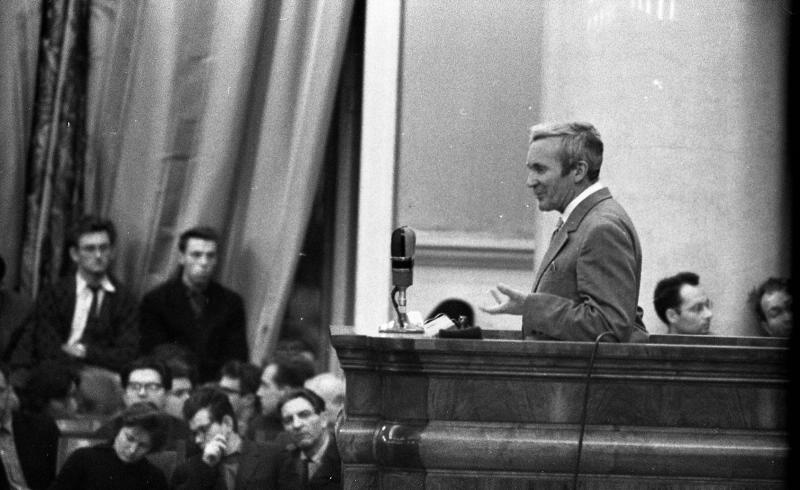
\includegraphics[height=0.40\textheight]{ch4_kolmogorov_1963.jpg}\\[1mm]
\imgcap{Kolmogorov la un curs la Moscova, 1963--1964}
\imgcredit{https://commons.wikimedia.org/wiki/File:\%D0\%9C\%D0\%B0\%D1\%82\%D0\%B5\%D0\%BC\%D0\%B0\%D1\%82\%D0\%B8\%D0\%BA_\%D0\%90\%D0\%BD\%D0\%B4\%D1\%80\%D0\%B5\%D0\%B9_\%D0\%9A\%D0\%BE\%D0\%BB\%D0\%BC\%D0\%BE\%D0\%B3\%D0\%BE\%D1\%80\%D0\%BE\%D0\%B2_\%D0\%B2_\%D0\%B0\%D1\%83\%D0\%B4\%D0\%B8\%D1\%82\%D0\%BE\%D1\%80\%D0\%B8\%D0\%B8.jpg}{Foto: Vsevolod Tarasevich (1963--1964); CC BY 4.0; Wikimedia Commons}
\end{column}
\end{columns}
\end{frame}

\begin{frame}{Evenimente, probabilitate condiționată, independență}
\itemsize{\footnotesize}
\begin{itemize}
    \item \textbf{Probabilitatea condiționată}: $P(A \mid B) = P(A \cap B)/P(B)$, pentru $P(B) > 0$
    \begin{itemize}
        \item $A, B$: două evenimente; $A \cap B$: au loc amîndouă
        \item în cuvinte: dintre cazurile în care are loc $B$, proporția celor în care are loc și $A$
    \end{itemize}
    \item \textbf{Regula lui Bayes}: $P(B \mid A) = P(A \mid B)P(B)/P(A)$
    \begin{itemize}
        \item $P(B)$: probabilitatea lui $B$ înainte de a afla $A$; $P(B \mid A)$: probabilitatea actualizată după ce observăm $A$
        \item inversează sensul condiționării: de la „semnal dată fiind criza” la „criză dat fiind semnalul”
    \end{itemize}
    \item Evenimente \textbf{independente}: $P(A \cap B) = P(A)P(B)$, adică $P(A \mid B) = P(A)$
    \begin{itemize}
        \item faptul că $B$ a avut loc nu schimbă probabilitatea lui $A$
    \end{itemize}
\end{itemize}
\end{frame}

\begin{frame}{Exemplu: zile de scădere consecutive}
\itemsize{\small}
\begin{itemize}
    \item S\&P 500, 2000--2026: $P(\text{zi de scădere}) = 46{,}3\%$
    \begin{itemize}
        \item după o zi de scădere: $P(\text{scădere} \mid \text{scădere ieri}) = 43{,}4\%$
        \item două zile de scădere la rînd: 20{,}1\% în date
        \item în ipoteza de independență: $P(\text{scădere})^2 = 21{,}4\%$, apropiat de date
    \end{itemize}
    \item BET: 50{,}0\% după o zi de scădere, față de 42{,}6\% după o zi de creștere
    \begin{itemize}
        \item semnul randamentului persistă de la o zi la alta
        \item o consecință a lichidității reduse: prețurile se ajustează la știri în mai multe zile
    \end{itemize}
\end{itemize}
\end{frame}

\begin{frame}{Recapitulare: de la jocuri la axiome}
\itemsize{\small}
\begin{itemize}
    \item Spațiul de probabilitate $(\Omega, \mathcal{F}, P)$ și trei axiome
    \item Valoare corectă = valoare așteptată: ideea lui Pascal și Fermat
    \item Probabilitatea condiționată măsoară cum schimbă informația șansele
\end{itemize}
\end{frame}


%=============================================================================
\section{Variabile aleatoare și distribuții}
%=============================================================================

\begin{frame}{Variabile aleatoare}
\itemsize{\footnotesize}
\begin{itemize}
    \item O \textbf{variabilă aleatoare} $X: \Omega \to \mathbb{R}$ asociază un număr fiecărui rezultat
    \begin{itemize}
        \item randamentul logaritmic de mîine, numărul zilelor de creștere dintr-o săptămînă, pierderea unui portofoliu
    \end{itemize}
    \item \textbf{Discretă}: un număr finit sau numărabil de valori $x_i$
    \begin{itemize}
        \item \textbf{PMF} (probability mass function, funcția de masă de probabilitate): $p(x_i) = P(X = x_i)$, cu $\sum_i p(x_i) = 1$
        \item $p(x_i)$: probabilitatea valorii $x_i$; probabilitățile tuturor valorilor însumează 1
    \end{itemize}
    \item \textbf{Continuă}: $P(a < X \le b) = \int_a^b f(x)\,dx$
    \begin{itemize}
        \item probabilitatea unui interval $(a, b]$ este aria de sub $f$ între $a$ și $b$
        \item $f$ este \textbf{PDF} (probability density function, densitatea de probabilitate): $f \ge 0$, iar aria totală $\int f = 1$
        \item un singur punct nu are arie: $P(X = x) = 0$ pentru orice $x$
    \end{itemize}
    \item Manual: \refFHH, secț.~3.1
\end{itemize}
\end{frame}

\begin{frame}{Funcția de repartiție și funcția cuantilă}
\itemsize{\small}
\begin{itemize}
    \item \textbf{CDF} (cumulative distribution function, funcția de repartiție): $F(x) = P(X \le x)$
    \begin{itemize}
        \item probabilitatea ca $X$ să nu depășească pragul $x$
        \item nedescrescătoare, continuă la dreapta, de la $F(-\infty) = 0$ la $F(\infty) = 1$
        \item pentru $X$ continuă, densitatea este derivata ei: $f = F'$
    \end{itemize}
    \item \textbf{Cuantila} de ordin $\alpha$: $q_\alpha = F^{-1}(\alpha) = \inf\{x : F(x) \ge \alpha\}$
    \begin{itemize}
        \item $\alpha \in (0, 1)$: o probabilitate; $q_\alpha$ este cel mai mic $x$ pentru care $P(X \le x) \ge \alpha$
        \item $F^{-1}$: funcția cuantilă, inversa funcției de repartiție; $\inf$: cea mai mică valoare a mulțimii
        \item mediana $= q_{0{,}5}$; cuantila de 1\% este randamentul depășit în 99\% din zile
    \end{itemize}
\end{itemize}
\end{frame}

\begin{frame}{VaR și funcția de repartiție empirică}
\itemsize{\small}
\begin{itemize}
    \item \textbf{VaR} (Value at Risk, valoarea expusă la risc) 1\%: $\text{VaR}_{1\%} = -q_{0{,}01}$
    \begin{itemize}
        \item $q_{0{,}01}$: cuantila de 1\% a randamentelor, un număr negativ
        \item semnul minus o transformă în pierdere: pierderea depășită cu probabilitatea 1\%
        \item estimarea și backtesting-ul: \sfmchlink{https://danpele.github.io/SFM/RO/Cursuri/capitol10_var_es_backtesting.pdf}{Capitolul 10}
    \end{itemize}
    \item \textbf{CDF empirică} a unui eșantion: $\hat F(x) = \frac1n \#\{t : r_t \le x\}$
    \begin{itemize}
        \item $r_1, \dots, r_n$: randamentele observate; $n$: volumul eșantionului
        \item $\#\{\cdot\}$: numărul de zile din mulțime; $\hat F(x)$ este proporția zilelor cu randamentul cel mult $x$
        \item căciula marchează o estimare calculată din date
    \end{itemize}
\end{itemize}
\end{frame}

\begin{frame}{O variabilă aleatoare discretă și una continuă}
\itemsize{\footnotesize}
\begin{center}
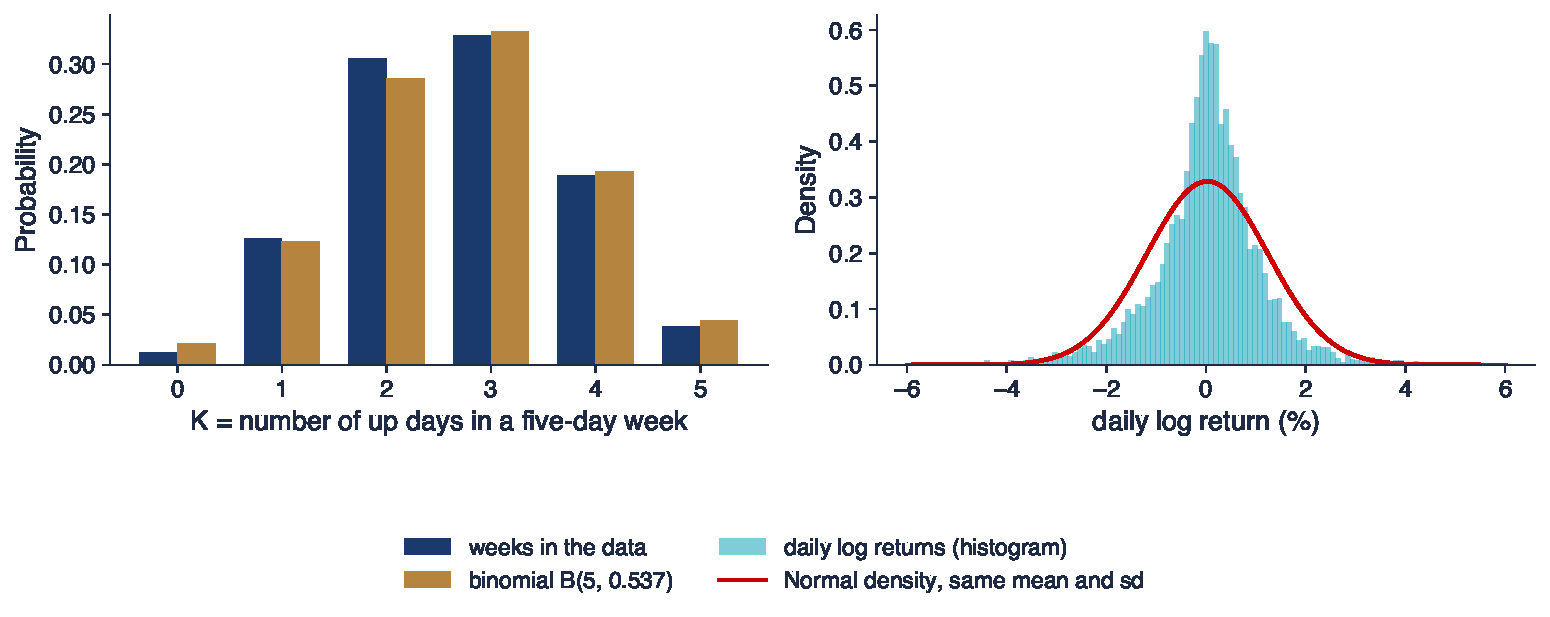
\includegraphics[width=0.97\textwidth,height=0.56\textheight,keepaspectratio]{sfm_ch4_random_variables.pdf}
\end{center}
\vspace{-0.25cm}
\begin{itemize}
    \item Stînga: $K$ = numărul zilelor de creștere dintr-o săptămînă completă a S\&P 500 (1\,144 de săptămîni)
    \begin{itemize}
        \item comparat cu $B(5, p)$, distribuția binomială: 5 zile, fiecare de creștere cu probabilitatea $p = 0{,}537$
        \item media 2{,}67 față de 2{,}69; varianța 1{,}16 față de 1{,}24
    \end{itemize}
    \item Dreapta: randamentele logaritmice zilnice, o variabilă aleatoare continuă; histograma estimează PDF
    \item Distribuția binomială se potrivește bine lui $K$; densitatea distribuției Normale nu surprinde nici vîrful, nici cozile randamentelor (\sfmchlink{https://danpele.github.io/SFM/RO/Cursuri/capitol2_distributii_clasice_fapte_stilizate.pdf}{Capitolul 2})
\end{itemize}
\sfmquantlet{Ch_04}{SFM_ch4_random_variables}
\end{frame}

\begin{frame}{CDF empirică și cuantila de 1\% a S\&P 500}
\itemsize{\footnotesize}
\begin{center}
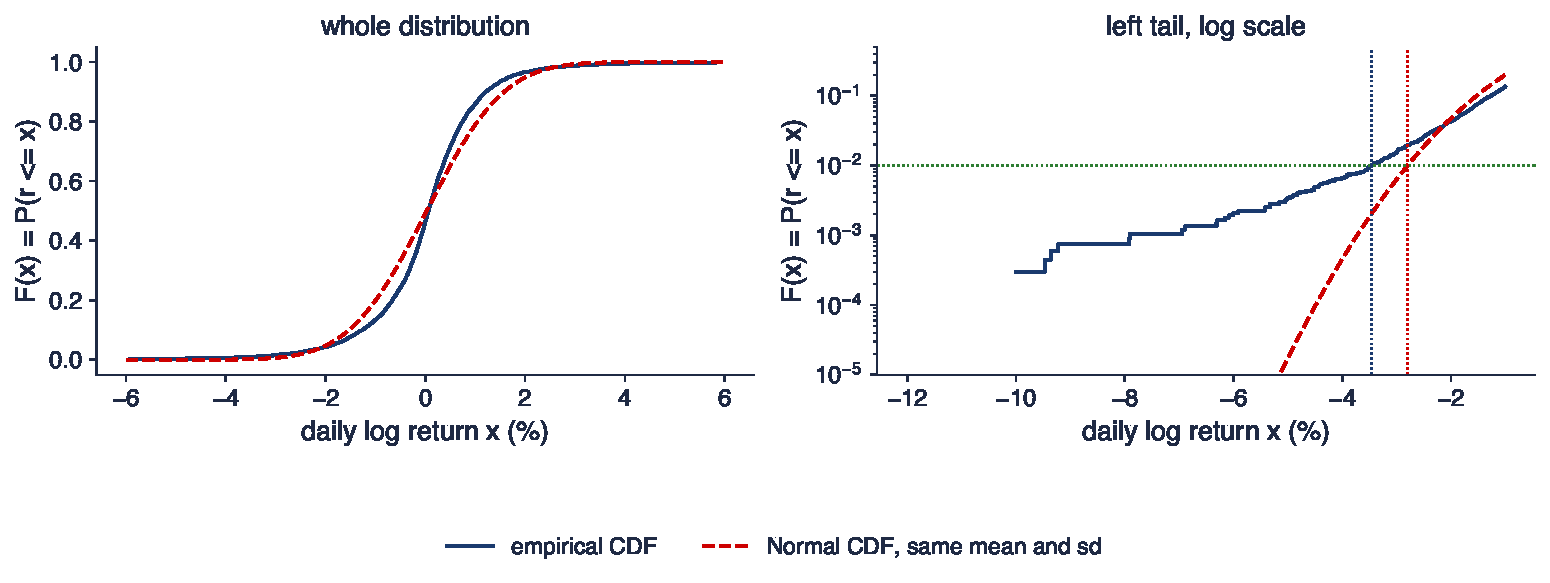
\includegraphics[width=0.97\textwidth,height=0.56\textheight,keepaspectratio]{sfm_ch4_cdf_quantile.pdf}
\end{center}
\vspace{-0.25cm}
\begin{itemize}
    \item $n = 6\,714$ zile; mediana $0{,}063\%$; în $\hat F(0) = 46{,}3\%$ din zile randamentul nu a fost pozitiv
    \item VaR 1\%: empiric 3{,}45\%, în distribuția Normală 2{,}80\%; $P(r < -3\%)$: 1{,}55\% față de 0{,}63\%
    \item $P(r < -5\%)$: 0{,}34\% în date, de 199 de ori mai mult decît în distribuția Normală ($1{,}7 \times 10^{-3}\%$)
\end{itemize}
\sfmquantlet{Ch_04}{SFM_ch4_random_variables}
\end{frame}

\begin{frame}{Recapitulare: variabile aleatoare}
\itemsize{\small}
\begin{itemize}
    \item PMF pentru variabile discrete, PDF pentru cele continue; CDF este definită pentru ambele
    \item Cuantilele inversează CDF; VaR 1\% este minus cuantila de 1\%
    \item Cozile CDF empirice sînt mult mai groase decît cele ale distribuției Normale
\end{itemize}
\end{frame}


%=============================================================================
\section{Speranța matematică și varianța}
%=============================================================================

\begin{frame}{Speranța matematică}
\itemsize{\footnotesize}
\begin{itemize}
    \item \textbf{Speranța matematică} (media): $E[X] = \sum_i x_i p(x_i)$ sau $E[X] = \int x f(x)\,dx$
    \begin{itemize}
        \item $x_i$, $p(x_i)$: valorile și probabilitățile lor; $f$: densitatea
        \item centrul de greutate al distribuției; există doar dacă $E|X| < \infty$ (nu și pentru Cauchy, \sfmchlink{https://danpele.github.io/SFM/RO/Cursuri/capitol3_distributii_alfa_stabile.pdf}{Capitolul 3})
    \end{itemize}
    \item A unei funcții: $E[g(X)] = \int g(x) f(x)\,dx$, fără a afla distribuția lui $g(X)$
    \item \textbf{Liniaritate}: $E[aX + bY + c] = aE[X] + bE[Y] + c$, întotdeauna (fără independență)
    \begin{itemize}
        \item $a, b, c$: constante; $X, Y$: oricare două variabile aleatoare
        \item randamentul așteptat al unui portofoliu este media ponderată a randamentelor așteptate
    \end{itemize}
    \item În general, $E[g(X)] \ne g(E[X])$
    \begin{itemize}
        \item Jensen: pentru $g$ convexă, $E[g(X)] \ge g(E[X])$; de exemplu, $E[e^X] > e^{E[X]}$
        \item sursa volatility drag din \sfmchlink{https://danpele.github.io/SFM/RO/Cursuri/capitol1_date_randamente_indicatori.pdf}{Capitolul 1}
    \end{itemize}
\end{itemize}
\end{frame}

\begin{frame}{Varianța și momentele}
\itemsize{\small}
\begin{itemize}
    \item \textbf{Varianța}: $\text{Var}(X) = E[(X - \mu)^2] = E[X^2] - \mu^2$
    \begin{itemize}
        \item $\mu = E[X]$; varianța este distanța pătratică medie față de medie
        \item abaterea standard $\sigma = \sqrt{\text{Var}(X)}$, în unitățile lui $X$; pentru randamente, este volatilitatea
    \end{itemize}
    \item $\text{Var}(aX + b) = a^2\,\text{Var}(X)$
    \begin{itemize}
        \item adăugarea unei constante $b$ nu schimbă riscul; înmulțirea cu $a$ înmulțește varianța cu $a^2$
    \end{itemize}
    \item Momentele: $E[X^k]$, pentru $k = 1, 2, \dots$
    \begin{itemize}
        \item asimetria $E[(X - \mu)^3]/\sigma^3$: lipsa de simetrie a distribuției (0 pentru distribuția Normală)
        \item boltirea $E[(X - \mu)^4]/\sigma^4$: egală cu 3 pentru distribuția Normală
        \item excesul de boltire = boltirea $-\,3$; pozitiv pentru cozi groase (\sfmchlink{https://danpele.github.io/SFM/RO/Cursuri/capitol2_distributii_clasice_fapte_stilizate.pdf}{Capitolul 2})
    \end{itemize}
\end{itemize}
\end{frame}

\begin{frame}{Exemplu lucrat: media și volatilitatea anuale}
\itemsize{\small}
\begin{itemize}
    \item S\&P 500, randamentele logaritmice zilnice $r_t$
    \begin{itemize}
        \item media zilnică $0{,}0247\%$, abaterea standard zilnică $\sigma = 1{,}213\%$
        \item $A = 252$: numărul de zile de tranzacționare pe an
    \end{itemize}
    \item Presupunem randamente zilnice i.i.d. (independente și identic distribuite)
    \begin{itemize}
        \item randamentul logaritmic anual este suma celor $A$ randamente zilnice: $\sum_{t=1}^{A} r_t$
    \end{itemize}
    \item Media: $E[\sum r_t] = A \times 0{,}0247 = 6{,}2\%$ pe an
    \begin{itemize}
        \item din liniaritatea speranței
    \end{itemize}
    \item Varianța: $\text{Var}(\sum r_t) = A\,\sigma^2$, pentru că toate covarianțele sînt zero
    \begin{itemize}
        \item volatilitatea anuală $\sigma\sqrt{A} = 1{,}213\sqrt{252} = 19{,}3\%$
        \item regula rădăcinii pătrate a timpului: pe $h$ perioade, volatilitatea crește cu $\sqrt{h}$
    \end{itemize}
\end{itemize}
\end{frame}

\begin{frame}{Frecvența zilelor de 4 sigma: marginea lui Cebîșev}
\itemsize{\small}
\begin{itemize}
    \item \textbf{Inegalitatea lui Cebîșev}: pentru orice $X$ cu varianță finită, $P(|X - \mu| \ge k\sigma) \le 1/k^2$
    \begin{itemize}
        \item $\mu$, $\sigma$: media și abaterea standard; $k > 1$: distanța față de medie, în abateri standard
        \item folosește doar media și varianța, deci este valabilă pentru orice distribuție
    \end{itemize}
    \item $k = 4$, S\&P 500, 2000--2026
    \begin{itemize}
        \item marginea Cebîșev: cel mult 6{,}25\% din zile
        \item distribuția Normală: 0{,}0063\%
        \item în date: 46 de zile, 0{,}69\%
    \end{itemize}
    \item Frecvența observată se află între cele două valori
    \begin{itemize}
        \item distribuția Normală este mult prea optimistă; cazul cel mai nefavorabil al lui Cebîșev este prea pesimist
    \end{itemize}
\end{itemize}
\end{frame}

\begin{frame}{Recapitulare: speranța și varianța}
\itemsize{\small}
\begin{itemize}
    \item Speranța este liniară; varianța se scalează cu pătratul
    \item Pentru randamente i.i.d., media crește cu $h$, iar volatilitatea cu $\sqrt{h}$
    \item Cebîșev mărginește probabilitățile din cozi pentru orice distribuție
\end{itemize}
\end{frame}


%=============================================================================
\section{Distribuții comune și dependență}
%=============================================================================

\begin{frame}{Distribuția comună și distribuțiile marginale}
\itemsize{\small}
\begin{itemize}
    \item \textbf{CDF comună}: $F(x, y) = P(X \le x, Y \le y)$
    \begin{itemize}
        \item probabilitatea ca ambele variabile să fie simultan sub pragurile lor
        \item pentru două randamente: ambele piețe scad sub nivelurile date în aceeași zi
    \end{itemize}
    \item CDF \textbf{marginală}: $F_X(x) = F(x, \infty)$
    \begin{itemize}
        \item distribuția lui $X$ singură, oricare ar fi valoarea lui $Y$
    \end{itemize}
    \item \textbf{PDF comună} $f(x, y)$: $P((X, Y) \in B) = \iint_B f(x, y)\,dx\,dy$
    \begin{itemize}
        \item $B$: o regiune din plan; probabilitatea este volumul de sub $f$ deasupra lui $B$
        \item densitatea marginală: $f_X(x) = \int f(x, y)\,dy$, prin integrare după $y$
    \end{itemize}
\end{itemize}
\end{frame}

\begin{frame}{Covarianța, corelația și varianța unei sume}
\itemsize{\footnotesize}
\begin{itemize}
    \item \textbf{Covarianța}: $\text{Cov}(X, Y) = E[(X - \mu_X)(Y - \mu_Y)] = E[XY] - \mu_X\mu_Y$
    \begin{itemize}
        \item $\mu_X$, $\mu_Y$: mediile; pozitivă cînd $X$ și $Y$ tind să fie simultan peste mediile lor
    \end{itemize}
    \item \textbf{Corelația}: $\rho = \text{Cov}(X, Y)/(\sigma_X\sigma_Y) \in [-1, 1]$
    \begin{itemize}
        \item covarianța împărțită la cele două abateri standard: un număr fără unitate de măsură
        \item măsoară doar dependența \textbf{liniară}; $|\rho| = 1$ dacă și numai dacă $Y = a + bX$
    \end{itemize}
    \item \textbf{Varianța unei sume}: $\text{Var}(aX + bY) = a^2\sigma_X^2 + b^2\sigma_Y^2 + 2ab\,\text{Cov}(X, Y)$
    \begin{itemize}
        \item $a, b$: constante (într-un portofoliu, ponderile); termenul de covarianță poate crește sau reduce riscul
        \item mai multe active: $\sigma_p^2 = w^\top \Sigma w$, cu $w$ vectorul ponderilor și $\Sigma$ matricea de covarianță
        \item $\sigma_p^2$: varianța portofoliului; $w^\top$: vectorul transpus
    \end{itemize}
\end{itemize}
\end{frame}

\begin{frame}{Distribuții comune ale randamentelor zilnice}
\itemsize{\footnotesize}
\begin{center}
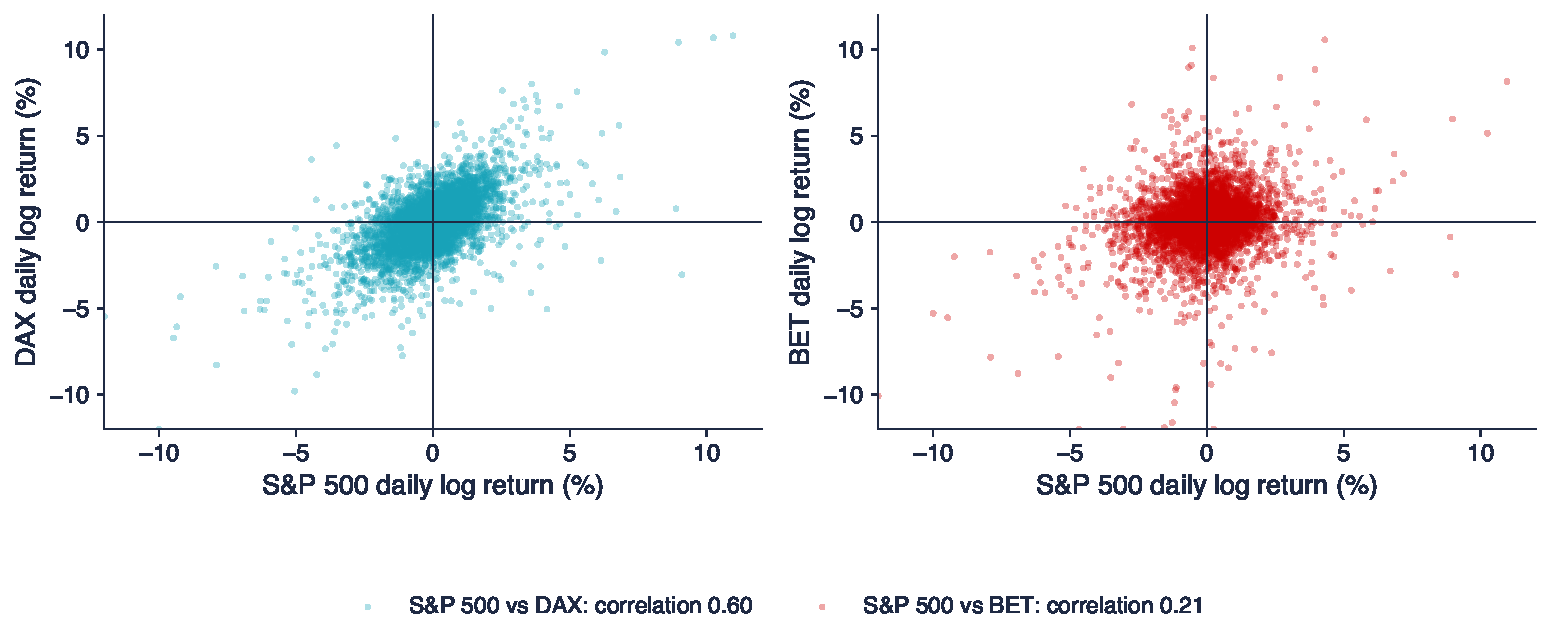
\includegraphics[width=0.97\textwidth,height=0.56\textheight,keepaspectratio]{sfm_ch4_joint.pdf}
\end{center}
\vspace{-0.25cm}
\begin{itemize}
    \item Doar zilele de tranzacționare comune: întîi se unesc prețurile, apoi se calculează randamentele ($n = 6\,605$ zile pentru S\&P 500 și DAX)
    \item S\&P 500 și DAX: $\rho = 0{,}60$; S\&P 500 și BET: $\rho = 0{,}21$
    \item Norul este eliptic în centru, dar zilele extreme apar simultan: crizele lovesc toate piețele deodată
\end{itemize}
\sfmquantlet{Ch_04}{SFM_ch4_dependence}
\end{frame}

\begin{frame}{Exemplu lucrat: un portofoliu 50/50 din S\&P 500 și DAX}
\itemsize{\footnotesize}
\begin{itemize}
    \item Abaterile standard zilnice: $\sigma_1 = 1{,}22\%$ (S\&P 500), $\sigma_2 = 1{,}43\%$ (DAX)
    \begin{itemize}
        \item covarianța $1{,}045$; corelația $0{,}60$
        \item ponderile $a = b = 0{,}5$, deci $a^2 = b^2 = 0{,}25$ și $2ab = 0{,}5$
    \end{itemize}
    \item $\sigma_p^2 = 0{,}25\sigma_1^2 + 0{,}25\sigma_2^2 + 2 \times 0{,}25\,\text{Cov} = 0{,}883 + 0{,}522 = 1{,}405$
    \begin{itemize}
        \item $\sigma_p = 1{,}19\%$, sub volatilitatea medie $1{,}32\%$: efectul diversificării
    \end{itemize}
    \item S\&P 500 și BET, corelație mai mică: $\sigma_p = 1{,}04\%$ față de media $1{,}33\%$
    \begin{itemize}
        \item cu cît corelația este mai mică, cu atît reducerea riscului este mai mare
    \end{itemize}
    \item Diversificarea funcționează doar prin $\rho < 1$
    \begin{itemize}
        \item într-un crah corelațiile cresc, exact cînd diversificarea ar fi necesară
    \end{itemize}
\end{itemize}
\end{frame}

\begin{frame}{Independență și necorelare}
\itemsize{\small}
\begin{itemize}
    \item $X$ și $Y$ sînt \textbf{independente} dacă $F(x, y) = F_X(x)F_Y(y)$ pentru orice $x, y$
    \begin{itemize}
        \item CDF comună este produsul CDF marginale
        \item atunci $E[g(X)h(Y)] = E[g(X)]E[h(Y)]$ pentru \textbf{toate} funcțiile $g, h$ (de exemplu, pătrate sau valori absolute)
    \end{itemize}
    \item Independente $\Rightarrow$ necorelate ($g, h$ = identitatea); reciproca este falsă
    \item Exemplu: $X \sim N(0, 1)$, $Y = X^2$
    \begin{itemize}
        \item $\text{Cov}(X, X^2) = E[X^3] = 0$: necorelate
        \item dar $Y$ este o funcție de $X$: complet dependente
    \end{itemize}
    \item Excepție: pentru variabile cu distribuție Normală comună (bivariată), necorelate $\Leftrightarrow$ independente
\end{itemize}
\end{frame}

\begin{frame}{Randamentele sînt necorelate, pătratele lor nu}
\itemsize{\scriptsize}
\begin{center}
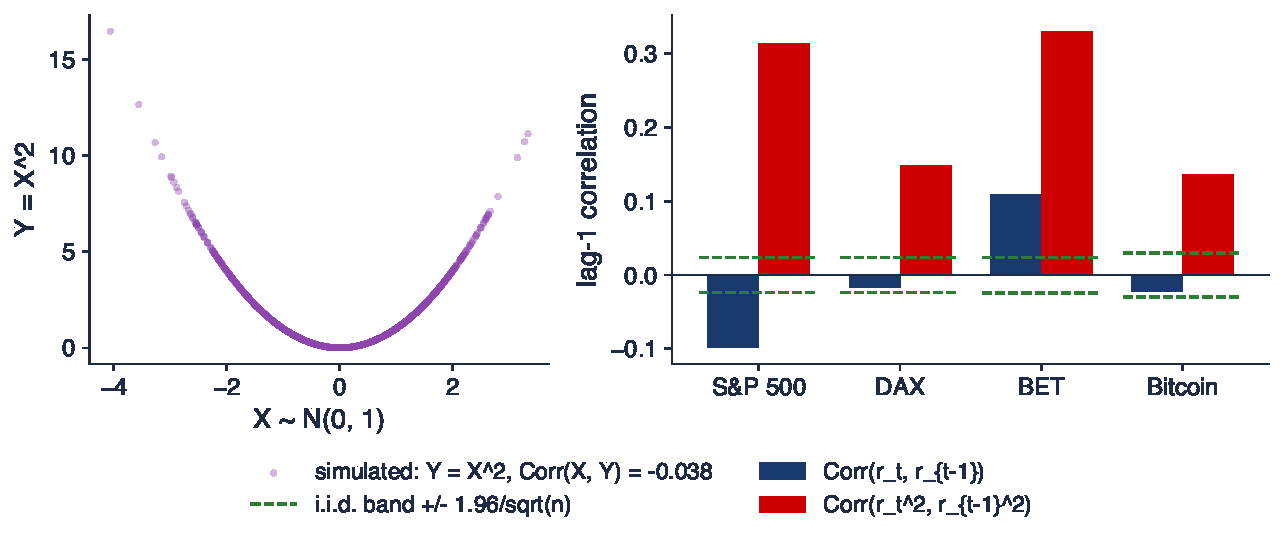
\includegraphics[width=0.97\textwidth,height=0.46\textheight,keepaspectratio]{sfm_ch4_uncorrelated_dependent.pdf}
\end{center}
\vspace{-0.25cm}
\begin{itemize}
    \item Stînga: $Y = X^2$ simulat, corelația de selecție $-0{,}038$, deși $Y$ este determinat de $X$
    \item Dreapta: $\text{Corr}(r_t, r_{t-1})$ este mică: S\&P 500 $-0{,}099$, DAX $-0{,}017$, Bitcoin $-0{,}022$
    \begin{itemize}
        \item $\text{Corr}(r_t^2, r_{t-1}^2)$ iese mult din bandă: $0{,}31$, $0{,}15$, $0{,}14$
        \item banda $\pm 1{,}96/\sqrt{n}$: valorile compatibile cu o corelație nulă, la pragul de 5\%
        \item valoarea negativă pentru S\&P 500 provine mai ales din zilele de criză
    \end{itemize}
    \item BET: $\text{Corr}(r_t, r_{t-1}) = 0{,}109$, un efect al lichidității reduse
\end{itemize}
\sfmquantlet{Ch_04}{SFM_ch4_dependence}
\end{frame}

\begin{frame}{Recapitulare: distribuții comune}
\itemsize{\small}
\begin{itemize}
    \item Covarianța intră în varianța oricărui portofoliu
    \item Independența implică necorelarea, nu invers
    \item Randamentele: aproape necorelate, dar pătratele lor sînt corelate, deci nu sînt independente
\end{itemize}
\end{frame}


%=============================================================================
\section{Speranța condiționată și varianța condiționată}
%=============================================================================

\begin{frame}{Speranța condiționată}
\itemsize{\footnotesize}
\begin{itemize}
    \item Densitatea condiționată: $f(y \mid x) = f(x, y)/f_X(x)$
    \begin{itemize}
        \item distribuția lui $Y$ după ce aflăm că $X = x$: densitatea comună rescalată prin cea marginală
    \end{itemize}
    \item \textbf{Speranța condiționată}: $E[Y \mid X = x] = \int y f(y \mid x)\,dy$
    \begin{itemize}
        \item media lui $Y$ calculată cu densitatea condiționată
        \item $E[Y \mid X]$ este o variabilă aleatoare, o funcție de $X$
    \end{itemize}
    \item Este cea mai bună prognoză a lui $Y$ pe baza lui $X$: minimizează $E[(Y - g(X))^2]$ dintre toate funcțiile $g$
    \begin{itemize}
        \item $E[(Y - g(X))^2]$: eroarea pătratică medie a prognozei $g(X)$
        \item pentru randamente: $E[r_t \mid \mathcal{F}_{t-1}]$, prognoza dată fiind toată informația $\mathcal{F}_{t-1}$ pînă ieri
    \end{itemize}
    \item \textbf{Proprietatea turnului} (legea speranțelor iterate): $E\big[E[Y \mid X]\big] = E[Y]$
    \begin{itemize}
        \item media prognozelor condiționate, pe toate valorile lui $X$, este media necondiționată
    \end{itemize}
\end{itemize}
\end{frame}

\begin{frame}{Varianța condiționată și legea varianței totale}
\itemsize{\small}
\begin{itemize}
    \item \textbf{Varianța condiționată}: $\text{Var}(Y \mid X) = E\big[(Y - E[Y \mid X])^2 \mid X\big]$
    \begin{itemize}
        \item dispersia lui $Y$ în jurul mediei condiționate, după ce $X$ este cunoscut
    \end{itemize}
    \item \textbf{Legea varianței totale}: $\text{Var}(Y) = E\big[\text{Var}(Y \mid X)\big] + \text{Var}\big(E[Y \mid X]\big)$
    \begin{itemize}
        \item $E[\text{Var}(Y \mid X)]$: varianța medie din interiorul grupurilor definite de $X$
        \item $\text{Var}(E[Y \mid X])$: cît de mult diferă mediile grupurilor între ele
        \item riscul total = varianța din interiorul grupurilor + varianța dintre grupuri
    \end{itemize}
\end{itemize}
\end{frame}

\begin{frame}{Exemplu lucrat: două regimuri}
\itemsize{\footnotesize}
\begin{itemize}
    \item $X$ = regimul pieței, $Y = r$ = randamentul zilnic (în \%)
    \begin{itemize}
        \item calm: probabilitatea $0{,}7$, media $0{,}05\%$, abaterea standard $0{,}8\%$
        \item agitat: probabilitatea $0{,}3$, media $-0{,}10\%$, abaterea standard $2\%$
    \end{itemize}
    \item Media (proprietatea turnului): $E[r] = 0{,}7 \times 0{,}05 + 0{,}3 \times (-0{,}10) = 0{,}005\%$
    \item Cele două componente ale varianței
    \begin{itemize}
        \item în interiorul regimurilor: $E[\text{Var}(r \mid X)] = 0{,}7 \times 0{,}8^2 + 0{,}3 \times 2^2 = 1{,}648$
        \item între regimuri: $\text{Var}(E[r \mid X]) = 0{,}7(0{,}05 - E[r])^2 + 0{,}3(-0{,}10 - E[r])^2 = 0{,}0047$
    \end{itemize}
    \item $\text{Var}(r) = 1{,}653$, abaterea standard $1{,}286\%$
    \begin{itemize}
        \item aproape tot riscul provine din diferența de varianță dintre regimuri, nu din diferența de medie
    \end{itemize}
\end{itemize}
\end{frame}

\begin{frame}{Randamentul de azi dată fiind mișcarea de ieri}
\itemsize{\footnotesize}
\begin{center}
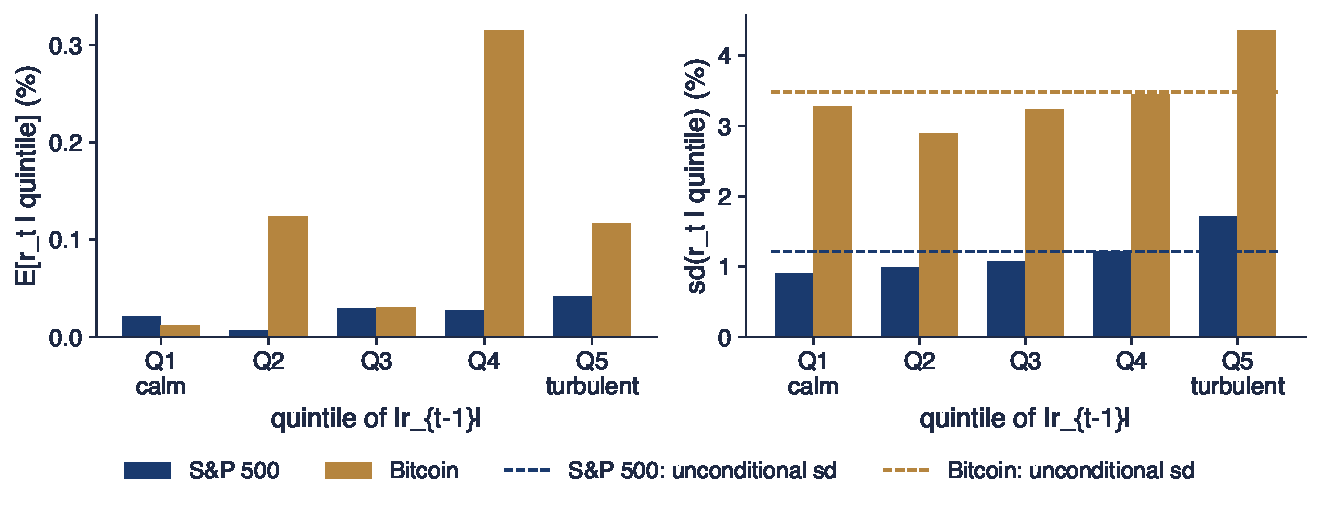
\includegraphics[width=0.97\textwidth,height=0.50\textheight,keepaspectratio]{sfm_ch4_conditional.pdf}
\end{center}
\vspace{-0.25cm}
\begin{itemize}
    \item Chintilele lui $|r_{t-1}|$: Q1 = cele mai calme 20\% dintre zilele de ieri, Q5 = cele mai agitate 20\%
    \item Media condiționată: între $0{,}006\%$ și $0{,}042\%$ pentru S\&P 500, fără un tipar util
    \item Abaterea standard condiționată: S\&P 500 de la 0{,}91\% (Q1) la 1{,}71\% (Q5), raportul Q5/Q1 1{,}88; Bitcoin, raportul 1{,}33
    \item Legea varianței totale, S\&P 500: 1{,}469 = 1{,}469 + 0{,}00013; componenta dintre grupuri reprezintă 0{,}01\% din total
\end{itemize}
\sfmquantlet{Ch_04}{SFM_ch4_dependence}
\end{frame}

\begin{frame}{De la varianța condiționată la GARCH}
\itemsize{\footnotesize}
\begin{itemize}
    \item Scriem randamentul ca $r_t = \mu_t + \sigma_t z_t$, cu $z_t$ i.i.d., media 0, varianța 1
    \begin{itemize}
        \item $\mu_t = E[r_t \mid \mathcal{F}_{t-1}]$: media condiționată, aproape constantă
        \item $\sigma_t^2 = \text{Var}(r_t \mid \mathcal{F}_{t-1})$: varianța condiționată, care se schimbă cu știrile
    \end{itemize}
    \item ARCH (autoregressive conditional heteroskedasticity) \refEngle: $\sigma_t^2 = \omega + \alpha r_{t-1}^2$
    \begin{itemize}
        \item varianța de azi este un nivel de bază plus o parte din pătratul randamentului de ieri
        \item $\omega > 0$: nivelul de bază; $\alpha \ge 0$: cît de mult crește varianța de azi după o mișcare mare ieri
    \end{itemize}
    \item GARCH \refBollerslev: $\sigma_t^2 = \omega + \alpha r_{t-1}^2 + \beta\sigma_{t-1}^2$ (\sfmchlink{https://danpele.github.io/SFM/RO/Cursuri/capitol9_modele_arch_garch.pdf}{Capitolul 9})
    \begin{itemize}
        \item $\beta \ge 0$: persistența; un $\beta$ mare menține mult timp o varianță ridicată
    \end{itemize}
    \item Este exact tiparul din grafic: un $|r_{t-1}|$ mare crește abaterea standard condiționată de azi
    \item Distribuția necondiționată este un amestec de distribuții cu diferite $\sigma_t$
    \begin{itemize}
        \item are cozi mai groase decît distribuția Normală, chiar dacă $z_t$ are distribuție Normală
    \end{itemize}
\end{itemize}
\end{frame}

\begin{frame}{Recapitulare: condiționare}
\itemsize{\small}
\begin{itemize}
    \item $E[Y \mid X]$ este cea mai bună prognoză; proprietatea turnului o readuce, în medie, la $E[Y]$
    \item Randamente: media condiționată aproape constantă, varianța condiționată puternic variabilă în timp
    \item Modelele ARCH și GARCH descriu dinamica lui $\sigma_t^2$
\end{itemize}
\end{frame}


%=============================================================================
\section{Legea numerelor mari și CLT}
%=============================================================================

\begin{frame}{Două teoreme limită}
\itemsize{\small}
\begin{itemize}
    \item \textbf{LLN} (law of large numbers, legea numerelor mari): pentru $X_i$ i.i.d. cu $E|X| < \infty$, $\bar X_n \to \mu$ cînd $n \to \infty$
    \begin{itemize}
        \item $\bar X_n = \frac1n\sum_{i=1}^n X_i$: media de selecție; $\mu = E[X]$: media adevărată
        \item motivul pentru care funcționează mediile, frecvențele și estimările Monte Carlo
    \end{itemize}
    \item \textbf{CLT} (central limit theorem, teorema limită centrală): cu varianță finită, $\sqrt{n}(\bar X_n - \mu)/\sigma \to N(0, 1)$ (\sfmchlink{https://danpele.github.io/SFM/RO/Cursuri/capitol2_distributii_clasice_fapte_stilizate.pdf}{Capitolul 2})
    \begin{itemize}
        \item media de selecție standardizată are, pentru $n$ mare, aproximativ distribuția Normală standard
        \item dă viteza de convergență: eroarea lui $\bar X_n$ este de circa $\sigma/\sqrt{n}$
        \item varianță infinită: sumele converg, în schimb, către legi $\alpha$-stabile (\sfmchlink{https://danpele.github.io/SFM/RO/Cursuri/capitol3_distributii_alfa_stabile.pdf}{Capitolul 3})
    \end{itemize}
    \item Ambele au nevoie de o formă de independență; randamentele dependente converg mai încet
\end{itemize}
\end{frame}

\begin{frame}{LLN pentru randamentul mediu: convergență lentă}
\itemsize{\footnotesize}
\begin{center}
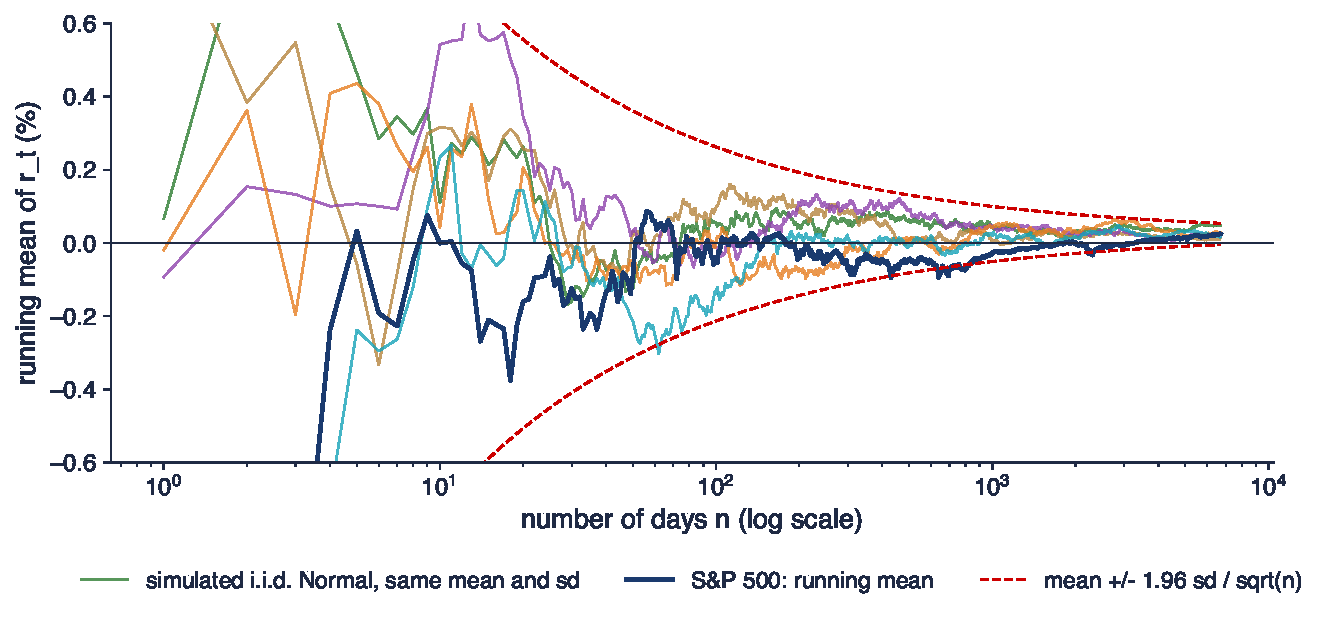
\includegraphics[width=0.97\textwidth,height=0.50\textheight,keepaspectratio]{sfm_ch4_lln.pdf}
\end{center}
\vspace{-0.25cm}
\begin{itemize}
    \item S\&P 500, 26{,}6 ani: media $0{,}0247\%$ pe zi, eroarea standard $\sigma/\sqrt{n} = 0{,}0148\%$
    \begin{itemize}
        \item $t$ = media / eroarea standard $= 1{,}67$; $|t| > 1{,}96$ ar indica o medie semnificativ diferită de 0, la pragul de 5\%
    \end{itemize}
    \item Media anuală 6{,}2\%, intervalul de încredere de 95\%: $[-1{,}1\%; 13{,}5\%]$
    \begin{itemize}
        \item nici 26 de ani de date nu ajung pentru a estima precis randamentul așteptat
        \item pentru $t = 3$, la această medie și volatilitate, ar fi nevoie de circa 86 de ani de date
    \end{itemize}
\end{itemize}
\sfmquantlet{Ch_04}{SFM_ch4_monte_carlo}
\end{frame}


%=============================================================================
\section{Numere aleatoare și Monte Carlo}
%=============================================================================

\begin{frame}{Ideea Monte Carlo}
\itemsize{\footnotesize}
\begin{itemize}
    \item Estimăm $\theta = E[g(X)]$ prin $\hat\theta_N = \frac1N\sum_{i=1}^N g(X_i)$, cu $X_i$ simulate
    \begin{itemize}
        \item $\theta$: mărimea necunoscută; $g$: o funcție de variabila simulată; $N$: numărul de simulări
        \item o probabilitate este o speranță: $P(A) = E[\mathbf{1}_A]$, cu $\mathbf{1}_A = 1$ dacă $A$ are loc și 0 altfel
        \item LLN face ca $\hat\theta_N \to \theta$; CLT dă eroarea $\text{sd}(g(X))/\sqrt{N}$, unde $\text{sd}$ este abaterea standard
    \end{itemize}
    \item Ulam și von Neumann au numit metoda după cazinoul din Monaco (Los Alamos, anii 1940) \refMU
    \item În finanțe \refGlasserman
    \begin{itemize}
        \item prețuri de opțiuni dependente de traiectorie, VaR-ul portofoliilor (\sfmchlink{https://danpele.github.io/SFM/RO/Cursuri/capitol10_var_es_backtesting.pdf}{Capitolul 10}), scenarii de stres
        \item orice speranță matematică fără formulă analitică
    \end{itemize}
    \item Două ingrediente: numere aleatoare uniforme și o metodă de a le transforma în extrageri din orice distribuție
\end{itemize}
\end{frame}

\begin{frame}{Numere pseudo-aleatoare: generatoare congruențiale liniare}
\itemsize{\small}
\begin{itemize}
    \item \textbf{LCG} (linear congruential generator, generator congruențial liniar): $x_{k+1} = (a x_k + c) \bmod M$, $u_k = x_k/M \in [0, 1)$
    \begin{itemize}
        \item fiecare număr întreg $x_{k+1}$ se calculează din precedentul, $x_k$
        \item $a$: multiplicatorul; $c$: incrementul; $M$: modulul; $\bmod M$: restul împărțirii la $M$
        \item $u_k$: numărul uniform din $[0, 1)$ obținut prin împărțirea la $M$
    \end{itemize}
    \item Determinist: aceeași sămînță $x_0$ dă același șir
    \begin{itemize}
        \item acest lucru face rezultatele reproductibile
        \item \textbf{perioada}: numărul de valori după care șirul se repetă; cel mult $M$
    \end{itemize}
    \item Generatoarele reale folosesc $M$ uriaș; perioada trebuie să fie mult mai lungă decît orice simulare
\end{itemize}
\end{frame}

\begin{frame}{Exemplu lucrat: un LCG cu $M = 16$}
\itemsize{\small}
\begin{itemize}
    \item SFErangen1: $a = 5$, $c = 1$, $M = 16$, $x_0 = 7$
    \begin{itemize}
        \item primul pas: $x_1 = (5 \times 7 + 1) \bmod 16 = 36 \bmod 16 = 4$
        \item șirul $x$: 7, 4, 5, 10, 3, 0, 1, 6, 15, 12, 13, 2, 11, 8, 9, 14, 7
    \end{itemize}
    \item Perioada 16, maximul posibil, $M$
    \begin{itemize}
        \item cu $a = 4$ șirul se blochează după un pas (perioada 1)
    \end{itemize}
    \item Nu ajunge ca distribuțiile marginale să fie uniforme
    \begin{itemize}
        \item numerele consecutive trebuie să pară și independente: graficul următor
    \end{itemize}
\end{itemize}
\end{frame}

\begin{frame}{RANDU: numerele aleatoare cad mai ales în plane (SFErandu)}
\itemsize{\footnotesize}
\begin{center}
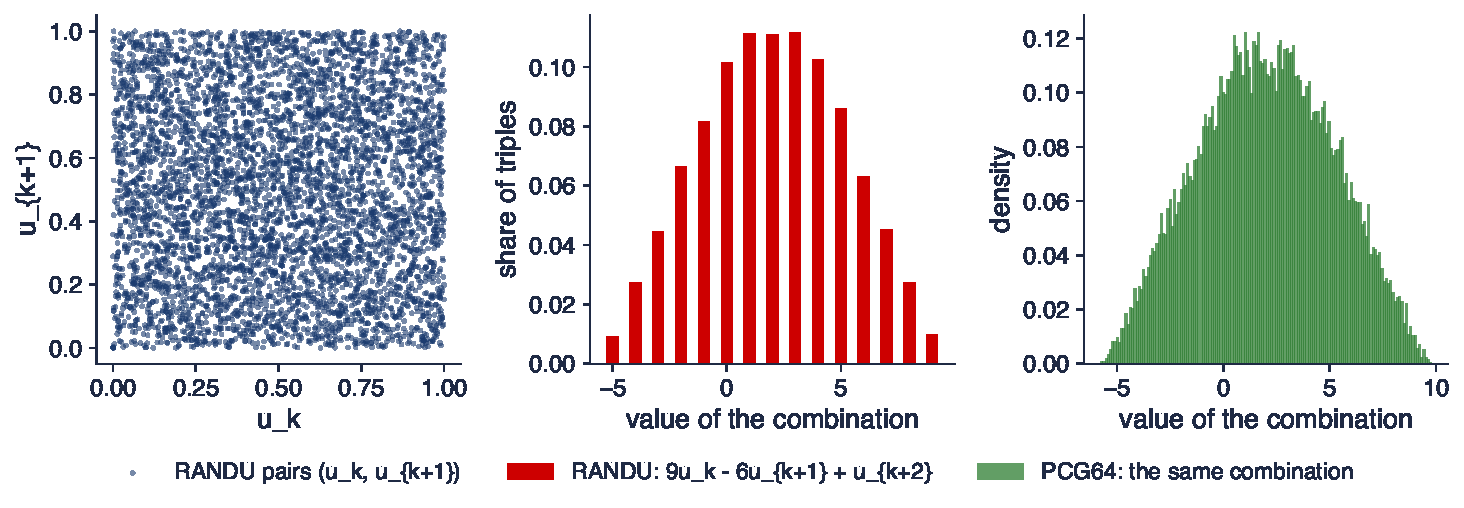
\includegraphics[width=0.97\textwidth,height=0.52\textheight,keepaspectratio]{sfm_ch4_randu.pdf}
\end{center}
\vspace{-0.25cm}
\begin{itemize}
    \item RANDU, IBM, anii 1960: $x_{k+1} = 65539\,x_k \bmod 2^{31}$; perechile par uniforme (stînga), corelația $0{,}003$
    \item Dar $9u_k - 6u_{k+1} + u_{k+2}$ ia doar 15 valori întregi, de la $-5$ la $9$: toate tripletele stau pe 15 plane \refMarsaglia
    \item Generatoare moderne: Mersenne Twister \refMT, PCG64 (implicit în NumPy, panoul din dreapta)
\end{itemize}
\sfmquantlet{Ch_04}{SFM_ch4_random_numbers}
\end{frame}

\begin{frame}{Metoda transformării inverse}
\itemsize{\footnotesize}
\begin{itemize}
    \item \textbf{Teoremă}: dacă $U \sim U(0, 1)$ și $F$ este o CDF, atunci $X = F^{-1}(U)$ are CDF $F$
    \begin{itemize}
        \item $U(0, 1)$: distribuția uniformă pe $[0, 1]$, deci $P(U \le u) = u$
        \item în cuvinte: un număr uniform, interpretat ca probabilitate, este transformat în cuantila de acel ordin
        \item demonstrație: $P(X \le x) = P(F^{-1}(U) \le x) = P(U \le F(x)) = F(x)$
    \end{itemize}
    \item Distribuția exponențială cu rata $\lambda > 0$: $F(x) = 1 - e^{-\lambda x}$, deci $X = -\ln(1 - U)/\lambda$
    \begin{itemize}
        \item se obține rezolvînd $u = F(x)$ în raport cu $x$; media este $1/\lambda$
        \item $\lambda = 2$, $u = 0{,}9$: $x = -\ln(0{,}1)/2 = 1{,}151$
    \end{itemize}
    \item Distribuția Normală: $X = \mu + \sigma\,\Phi^{-1}(U)$
    \begin{itemize}
        \item $\Phi^{-1}$: funcția cuantilă a distribuției $N(0, 1)$; $\mu$, $\sigma$: media și abaterea standard dorite
    \end{itemize}
    \item Pentru date reale: folosim funcția cuantilă empirică $\hat F^{-1}$
    \begin{itemize}
        \item adică reeșantionăm zilele trecute: simularea istorică și bootstrap-ul
    \end{itemize}
\end{itemize}
\end{frame}

\begin{frame}{Transformarea inversă: extrageri exponențiale, Normale și istorice}
\itemsize{\footnotesize}
\begin{center}
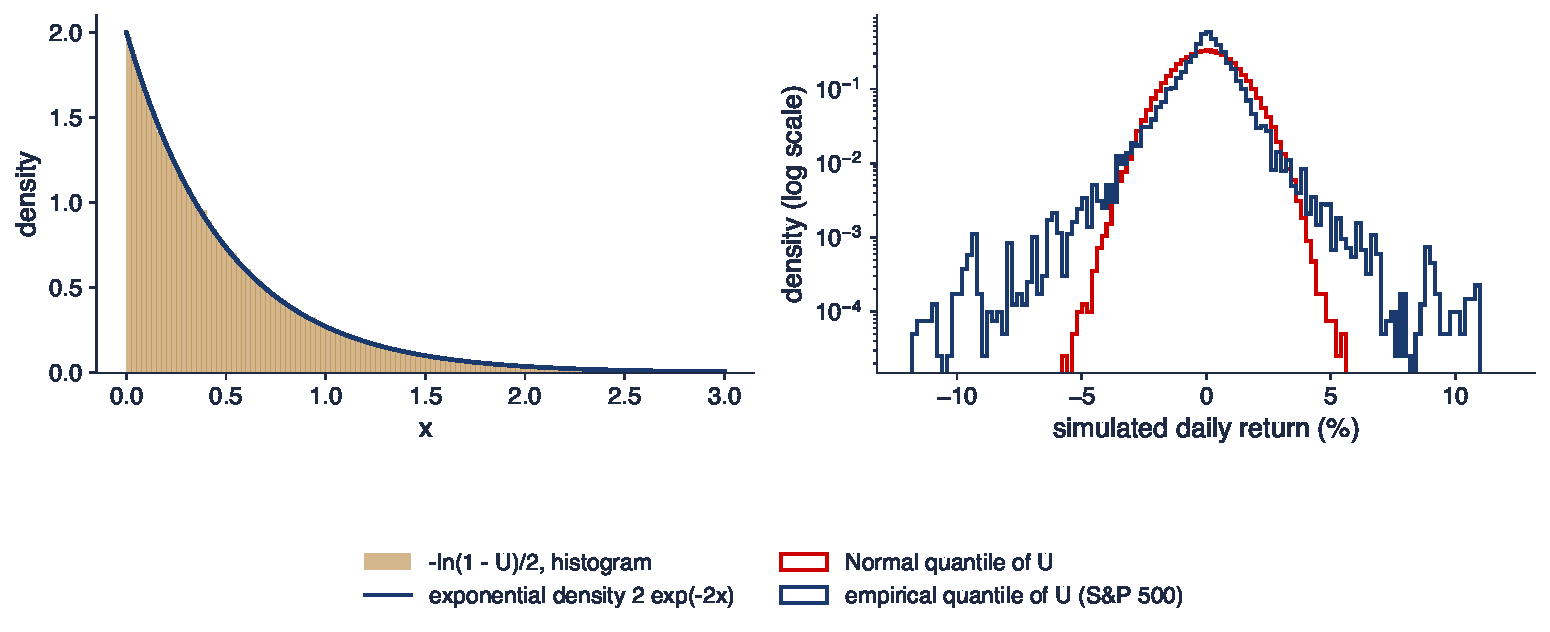
\includegraphics[width=0.97\textwidth,height=0.52\textheight,keepaspectratio]{sfm_ch4_inverse_transform.pdf}
\end{center}
\vspace{-0.25cm}
\begin{itemize}
    \item Stînga: 200\,000 de extrageri $-\ln(1 - U)/2$ urmează densitatea exponențială; media de selecție 0{,}500 (teoretic $1/\lambda = 0{,}5$)
    \item Dreapta: aceleași numere uniforme trecute prin funcția cuantilă a distribuției Normale și prin cea empirică a S\&P 500
    \item Extrageri sub $-5\%$: 0{,}0035\% din cele Normale față de 0{,}34\% din cele istorice (în date: 0{,}34\%); cea mai mică extragere: $-5{,}7\%$ față de $-12{,}7\%$
\end{itemize}
\sfmquantlet{Ch_04}{SFM_ch4_random_numbers}
\end{frame}

\begin{frame}{Exemplu lucrat: probabilitatea unei pierderi lunare prin Monte Carlo (1/2)}
\itemsize{\small}
\begin{itemize}
    \item Modelul: randamentele logaritmice zilnice ale S\&P 500, i.i.d. $N(0{,}0247; 1{,}213^2)$, în \%
    \begin{itemize}
        \item $N(m, s^2)$: distribuția Normală cu media $m$ și varianța $s^2$
    \end{itemize}
    \item Evenimentul: randamentul logaritmic pe 21 de zile (o lună) este sub $-10\%$
    \begin{itemize}
        \item $p$: probabilitatea lui, mărimea căutată
    \end{itemize}
    \item Exact: suma a 21 de randamente Normale i.i.d. este $N(0{,}519; 5{,}56^2)$
    \begin{itemize}
        \item media $21 \times 0{,}0247$, abaterea standard $1{,}213\sqrt{21}$
        \item standardizăm: $z = (-10 - 0{,}519)/5{,}56 = -1{,}892$
        \item $p = \Phi(z) = 2{,}922\%$, cu $\Phi$ funcția de repartiție a distribuției $N(0, 1)$
    \end{itemize}
\end{itemize}
\end{frame}

\begin{frame}{Exemplu lucrat: probabilitatea unei pierderi lunare prin Monte Carlo (2/2)}
\itemsize{\small}
\begin{itemize}
    \item Monte Carlo: simulăm $N$ luni; $\hat p_N$ = ponderea lunilor simulate sub $-10\%$
    \begin{itemize}
        \item eroarea standard $\sqrt{p(1 - p)/N}$: distanța tipică dintre $\hat p_N$ și $p$
    \end{itemize}
    \item Rezultate
    \begin{itemize}
        \item $N = 1\,000$: $3{,}000\%$ (eroarea standard 0{,}533\%)
        \item $N = 100\,000$: $2{,}901\%$ (eroarea standard 0{,}053\%)
        \item o precizie de 10 ori mai mare cere de 100 de ori mai multe simulări
    \end{itemize}
    \item Pentru o eroare relativă de 10\%, la nivelul de încredere de 95\%: $N \approx 1{,}96^2(1 - p)/(0{,}1^2 p) = 12\,762$
    \begin{itemize}
        \item se obține din $1{,}96 \times \sqrt{p(1 - p)/N} = 0{,}1\,p$: semilățimea intervalului este 10\% din $p$
        \item un eveniment rar cere multe simulări
    \end{itemize}
\end{itemize}
\end{frame}

\begin{frame}{Monte Carlo converge cu viteza $1/\sqrt{N}$}
\itemsize{\footnotesize}
\begin{center}
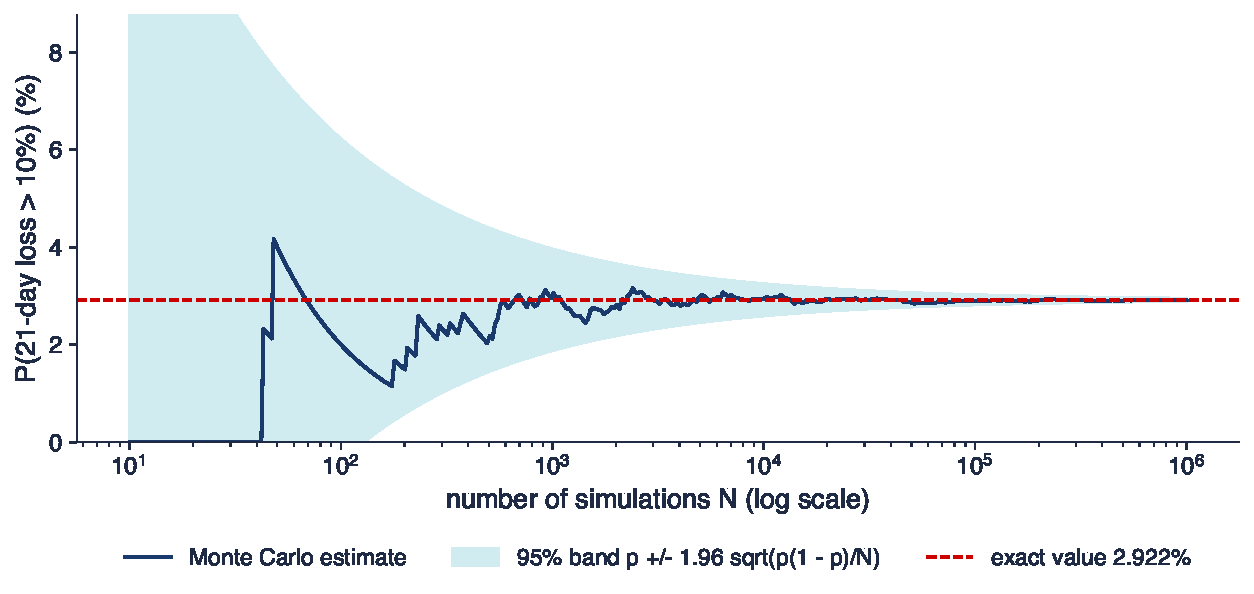
\includegraphics[width=0.97\textwidth,height=0.56\textheight,keepaspectratio]{sfm_ch4_monte_carlo.pdf}
\end{center}
\vspace{-0.25cm}
\begin{itemize}
    \item Pentru $N$ mic estimarea fluctuează mult, apoi intră în banda de 95\%, care se îngustează ca $1/\sqrt{N}$
    \item $N = 10^6$: $2{,}926\%$ față de valoarea exactă 2{,}922\%, eroarea standard 0{,}017\%
    \item Un $N$ mare reduce eroarea de simulare, nu și eroarea de model: Seminarul 4 (B3) repetă calculul cu zile reeșantionate
\end{itemize}
\sfmquantlet{Ch_04}{SFM_ch4_monte_carlo}
\end{frame}

\begin{frame}{Recapitulare: numere aleatoare și Monte Carlo}
\itemsize{\small}
\begin{itemize}
    \item Generatoarele pseudo-aleatoare sînt deterministe; verificați-le în mai multe dimensiuni
    \item $F^{-1}(U)$ transformă numerele uniforme în orice distribuție, inclusiv cea empirică
    \item Eroarea Monte Carlo $\propto 1/\sqrt{N}$; raportați-o întotdeauna
\end{itemize}
\end{frame}


%=============================================================================
\section{Modelul binomial}
%=============================================================================

\begin{frame}{Procesul binomial}
\itemsize{\footnotesize}
\begin{itemize}
    \item În fiecare perioadă prețul se înmulțește cu $u$ (creștere), cu probabilitatea $p$, sau cu $d < u$ (scădere), cu probabilitatea $1 - p$
    \begin{itemize}
        \item $u$, $d$: factorii de creștere și de scădere (de exemplu, $u = 1{,}2$: $+20\%$); perioadele sînt independente
    \end{itemize}
    \item După $n$ pași, dintre care $K$ creșteri: $S_n = S_0 u^K d^{n - K}$
    \begin{itemize}
        \item $S_0$: prețul inițial; $K \sim B(n, p)$: numărul de creșteri are distribuție binomială
        \item $\ln S_n = \ln S_0 + K\ln u + (n - K)\ln d$: un mers aleator în prețurile logaritmice (secțiunea 9)
    \end{itemize}
    \item $E[S_n] = S_0\,(pu + (1 - p)d)^n$, pentru că pașii sînt independenți
    \begin{itemize}
        \item $pu + (1 - p)d$: factorul de creștere așteptat al unui pas
        \item baza modelului binomial de evaluare a opțiunilor \refCRR; manual: \refFHH, cap.~7
    \end{itemize}
\end{itemize}
\end{frame}

\begin{frame}{Exemplu lucrat: un arbore cu doi pași}
\itemsize{\footnotesize}
\begin{itemize}
    \item $S_0 = 100$, $u = 1{,}2$, $d = 0{,}8$, $p = 0{,}6$
    \item Valorile finale și probabilitățile lor
    \begin{itemize}
        \item $uu$: 144 cu $p^2 = 0{,}36$; $ud$ sau $du$: 96 cu $2p(1-p) = 0{,}48$; $dd$: 64 cu $(1-p)^2 = 0{,}16$
    \end{itemize}
    \item $E[S_2] = 100 \times (0{,}6 \times 1{,}2 + 0{,}4 \times 0{,}8)^2 = 100 \times 1{,}04^2 = 108{,}16$
    \item $P(S_2 < 100) = 0{,}48 + 0{,}16 = 0{,}64$
    \begin{itemize}
        \item o creștere și o scădere, în orice ordine, aduc o pierdere, pentru că $ud = 0{,}96 < 1$
    \end{itemize}
    \item Cu $p^* = (1 - d)/(u - d) = 0{,}50$ prețul este un joc echitabil: $E[S_{t+1} \mid S_t] = S_t$ (secțiunea 9)
    \begin{itemize}
        \item $p^*$ este soluția ecuației $p^*u + (1 - p^*)d = 1$: factorul de creștere așteptat al unui pas este 1
    \end{itemize}
\end{itemize}
\end{frame}

\begin{frame}{Calibrarea arborelui pe o piață (Cox--Ross--Rubinstein)}
\itemsize{\footnotesize}
\begin{itemize}
    \item \textbf{CRR} (Cox--Ross--Rubinstein) cu pasul $\Delta t$: $u = e^{\sigma\sqrt{\Delta t}}$, $d = 1/u$, $p = (e^{\mu\Delta t} - d)/(u - d)$
    \begin{itemize}
        \item $\Delta t$: lungimea unui pas, în ani; $\mu$: tendința anuală (drift); $\sigma$: volatilitatea anuală
        \item $d = 1/u$: o creștere urmată de o scădere readuce prețul la valoarea inițială
        \item alese astfel încît media și varianța fiecărui pas să corespundă unei piețe cu tendința $\mu$ și volatilitatea $\sigma$
    \end{itemize}
    \item S\&P 500, 2000--2026: $\sigma = 19{,}26\%$, $\mu = 8{,}08\%$ pe an; pași zilnici, $\Delta t = 1/252$
    \begin{itemize}
        \item $u = 1{,}0122$, $d = 0{,}9879$, $p = 0{,}5102$
    \end{itemize}
    \item Cînd $\Delta t \to 0$, $\ln S_T$ devine Normal (CLT aplicată lui $K$)
    \begin{itemize}
        \item $T$: orizontul; arborele converge către GBM (secțiunea 10)
    \end{itemize}
\end{itemize}
\end{frame}

\begin{frame}{Traiectorii binomiale și limita lognormală (SFEBinomp)}
\itemsize{\footnotesize}
\begin{center}
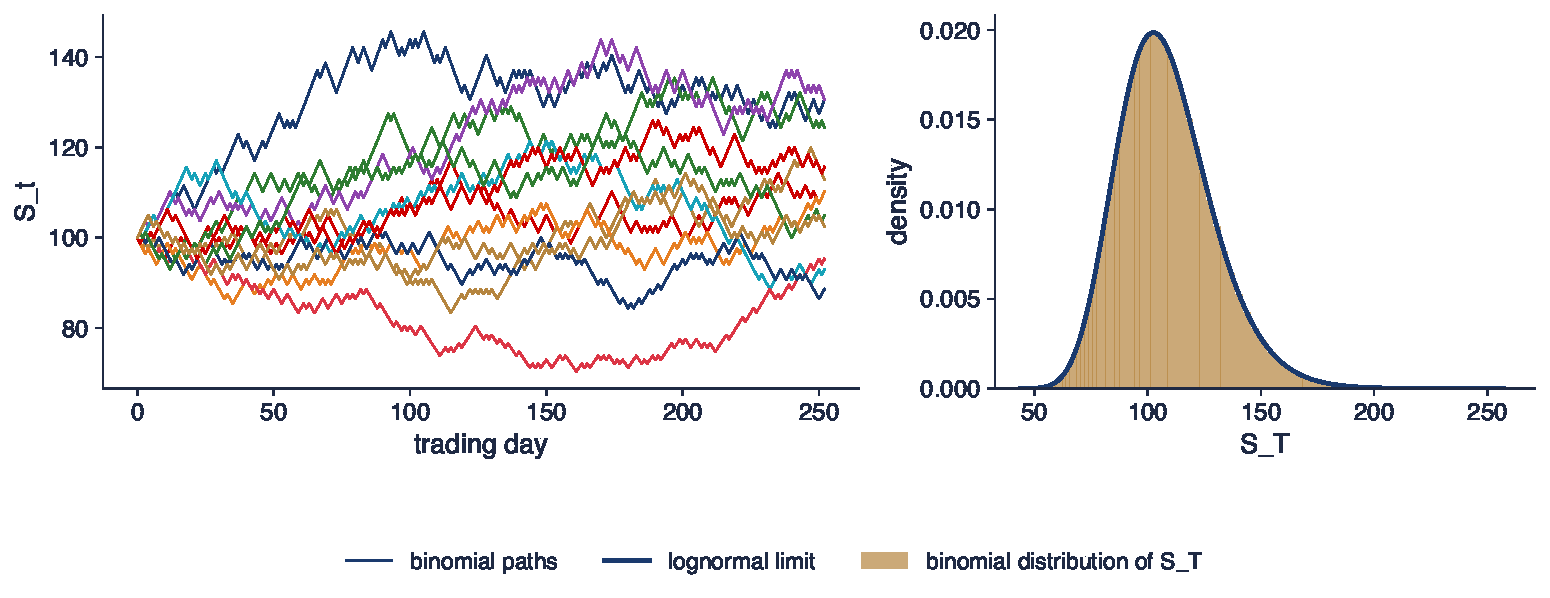
\includegraphics[width=0.97\textwidth,height=0.46\textheight,keepaspectratio]{sfm_ch4_binomial.pdf}
\end{center}
\vspace{-0.25cm}
\begin{itemize}
    \item Stînga: 12 traiectorii pe un an, cu pași zilnici, $S_0 = 100$
    \item Dreapta: distribuția lui $S_T$ după 252 de pași ($T = 1$ an); $E[S_T] = 108{,}42$ $= 100e^{\mu}$
    \begin{itemize}
        \item cuantila de 5\%: 78{,}5, față de 77{,}5 în limita lognormală
    \end{itemize}
    \item $P(S_T < 100)$: 39{,}7\% în modelul binomial, față de 37{,}3\% în cel lognormal
    \begin{itemize}
        \item valoarea exactă $S_T = 100$ are probabilitate pozitivă, pe care modelul binomial o plasează de o singură parte
    \end{itemize}
\end{itemize}
\sfmquantlet{Ch_04}{SFM_ch4_binomial}
\end{frame}

\begin{frame}{Recapitulare: modelul binomial}
\itemsize{\small}
\begin{itemize}
    \item Creștere sau scădere în fiecare perioadă: $S_n = S_0 u^K d^{n-K}$ cu $K$ binomial
    \item CRR reproduce $\mu$ și $\sigma$; limita este lognormală
    \item Un $p^*$ special transformă prețul într-un joc echitabil: cheia evaluării opțiunilor
\end{itemize}
\end{frame}


%=============================================================================
\section{Procese stochastice în timp discret}
%=============================================================================

\begin{frame}{Procese stochastice și informație}
\itemsize{\small}
\begin{itemize}
    \item Un \textbf{proces stochastic} $\{X_t\}$: o familie de variabile aleatoare indexate după timp
    \begin{itemize}
        \item o realizare = o traiectorie; o serie de prețuri este o singură traiectorie a procesului
    \end{itemize}
    \item $\mathcal{F}_t$: informația disponibilă la momentul $t$ (prețuri trecute, știri)
    \begin{itemize}
        \item crește cu $t$: nimic nu se uită (o \textbf{filtrare})
    \end{itemize}
    \item \textbf{Staționar (slab)}: $E[X_t]$ și $\text{Cov}(X_t, X_{t+h})$ nu depind de $t$
    \begin{itemize}
        \item $h$: lagul dintre două momente; media și dependența arată la fel la orice moment
        \item randamentele: aproximativ da; prețurile: nu
    \end{itemize}
    \item Manual: \refFHH, cap.~4 și secț.~11.3
\end{itemize}
\end{frame}

\begin{frame}{Zgomotul alb și mersul aleator}
\itemsize{\footnotesize}
\begin{itemize}
    \item \textbf{Zgomot alb}: $E[\varepsilon_t] = 0$, $\text{Var}(\varepsilon_t) = \sigma^2$, $\text{Cov}(\varepsilon_t, \varepsilon_s) = 0$ pentru $t \ne s$
    \begin{itemize}
        \item $\varepsilon_t$: șocul de la momentul $t$; medie zero, varianță constantă $\sigma^2$, necorelat între momente diferite
        \item zgomotul i.i.d. este o condiție mai tare: $\varepsilon_t$ sînt independente, nu doar necorelate
    \end{itemize}
    \item \textbf{Mers aleator}: $S_t = S_{t-1} + \mu + \varepsilon_t = S_0 + \mu t + \sum_{s=1}^t \varepsilon_s$
    \begin{itemize}
        \item fiecare pas adaugă tendința (drift-ul) $\mu$ și un șoc nou; $S_0$: valoarea de pornire
        \item $E[S_t] = S_0 + \mu t$; $\text{Var}(S_t) = t\sigma^2$ crește cu $t$: nestaționar
        \item simulat cu $\sigma = 1$: varianța 10{,}1; 49{,}8; 100{,}9 la $t = 10, 50, 100$
    \end{itemize}
    \item Dacă prețurile logaritmice urmează un mers aleator, randamentele sînt zgomot alb
    \begin{itemize}
        \item ipoteza de referință din \sfmchlink{https://danpele.github.io/SFM/RO/Cursuri/capitol7_piete_eficiente_mers_aleator_vr.pdf}{Capitolul 7} (piețe eficiente)
    \end{itemize}
\end{itemize}
\end{frame}

\begin{frame}{Martingale}
\itemsize{\footnotesize}
\begin{itemize}
    \item $\{X_t\}$ este un \textbf{martingal} dacă $E|X_t| < \infty$ și $E[X_{t+1} \mid \mathcal{F}_t] = X_t$
    \begin{itemize}
        \item $E|X_t| < \infty$: media există; $\mathcal{F}_t$: informația pînă la momentul $t$
        \item un joc echitabil: cea mai bună prognoză pentru mîine este valoarea de azi
    \end{itemize}
    \item O \textbf{diferență de martingal}: $\varepsilon_t = X_t - X_{t-1}$ cu $E[\varepsilon_t \mid \mathcal{F}_{t-1}] = 0$
    \begin{itemize}
        \item variația nu poate fi prevăzută pe baza trecutului
    \end{itemize}
    \item Exemple
    \begin{itemize}
        \item un mers aleator fără tendință; $S_t^2 - t\sigma^2$ pentru același mers; prețul binomial cu $p^*$
    \end{itemize}
    \item Martingal $\ne$ creșteri i.i.d.: \textbf{varianța} condiționată se poate schimba, ca în GARCH
    \begin{itemize}
        \item forma slabă a ipotezei pieței eficiente \refFama: randamentele în exces (peste dobînda fără risc) sînt o diferență de martingal
    \end{itemize}
\end{itemize}
\end{frame}

\begin{frame}{Procesul AR(1)}
\itemsize{\footnotesize}
\begin{itemize}
    \item \textbf{AR(1)} (autoregresiv de ordinul 1): $X_t = c + \phi X_{t-1} + \varepsilon_t$, $\varepsilon_t$ zgomot alb
    \begin{itemize}
        \item valoarea de azi este o constantă, plus o fracțiune $\phi$ din valoarea de ieri, plus un șoc nou
        \item $c$: constanta; $\phi$: persistența; $\sigma^2$: varianța lui $\varepsilon_t$
        \item $\phi = 0$: zgomot alb; $\phi = 1$, $c = \mu$: mers aleator
    \end{itemize}
    \item Staționar dacă și numai dacă $|\phi| < 1$; atunci
    \begin{itemize}
        \item media $c/(1 - \phi)$, varianța $\sigma^2/(1 - \phi^2)$
        \item autocorelația la lagul $h$: $\rho(h) = \text{Corr}(X_t, X_{t-h}) = \phi^h$, cu scădere geometrică
        \item timpul de înjumătățire al unui șoc: $\ln 0{,}5/\ln\phi$ perioade, timpul după care jumătate din șoc a dispărut
    \end{itemize}
    \item Utilizări
    \begin{itemize}
        \item dobînzi și spread-uri (revenire la medie)
        \item pătratele randamentelor se comportă ca un AR persistent, ceea ce duce la GARCH
    \end{itemize}
\end{itemize}
\end{frame}

\begin{frame}{Procesul AR(1): simulare}
\itemsize{\small}
\begin{itemize}
    \item Simulat cu $\sigma = 1$, $\phi = 0{,}5$
    \begin{itemize}
        \item varianța 1{,}34 (teoretic $1/(1 - 0{,}5^2) = 1{,}33$)
        \item $\rho(5) = 0{,}034$ (teoretic $0{,}5^5 = 0{,}031$); timpul de înjumătățire 1{,}0 perioade
    \end{itemize}
    \item Simulat cu $\sigma = 1$, $\phi = 0{,}95$
    \begin{itemize}
        \item varianța 10{,}20 (teoretic 10{,}26)
        \item $\rho(5) = 0{,}772$; timpul de înjumătățire 13{,}5 perioade
    \end{itemize}
    \item Cu cît $\phi$ este mai aproape de 1, cu atît varianța este mai mare și un șoc se stinge mai încet
\end{itemize}
\end{frame}

\begin{frame}{Zgomot alb, AR(1) și mers aleator, aceleași șocuri}
\itemsize{\footnotesize}
\begin{center}
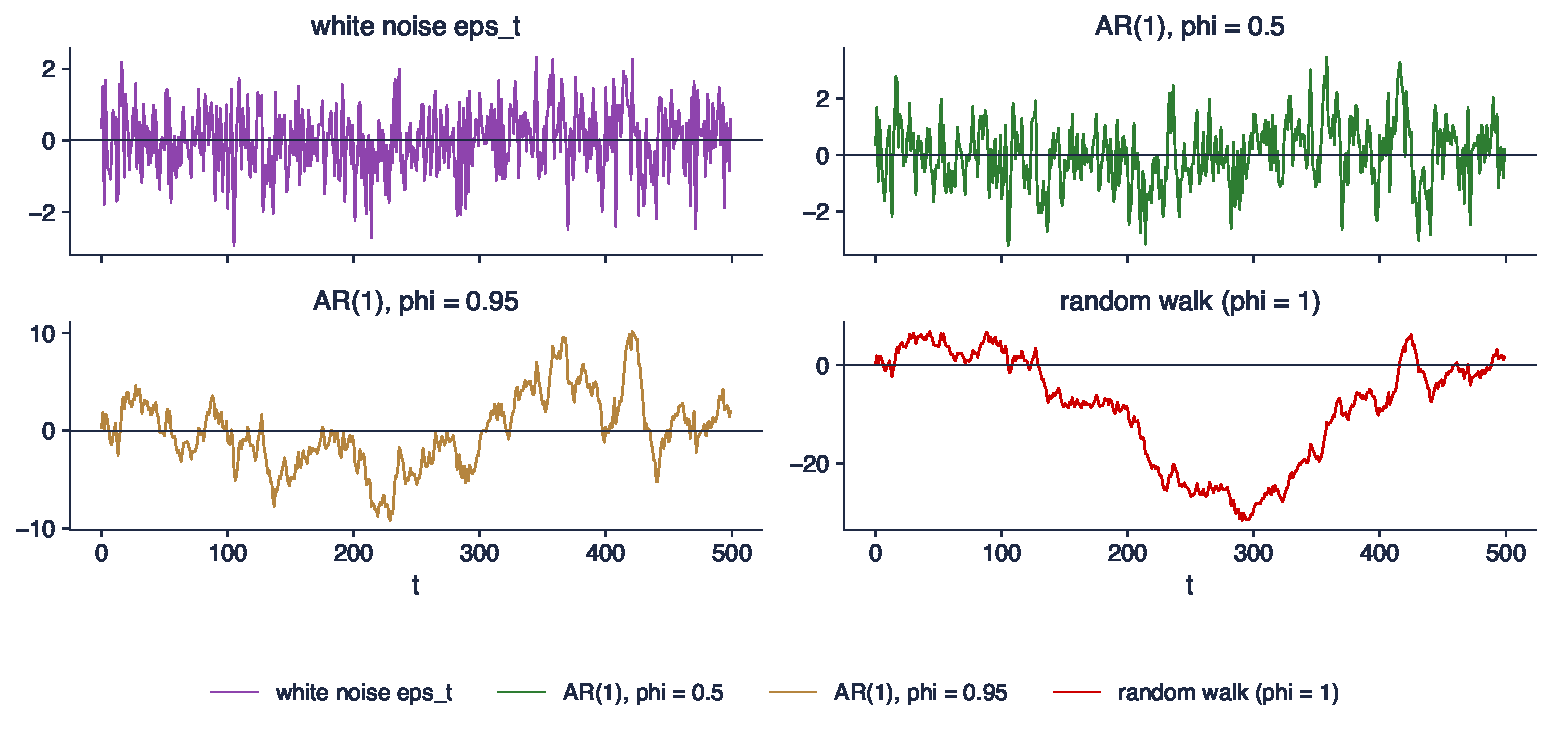
\includegraphics[width=0.97\textwidth,height=0.58\textheight,keepaspectratio]{sfm_ch4_processes.pdf}
\end{center}
\vspace{-0.25cm}
\begin{itemize}
    \item Cu cît $\phi$ este mai mare, cu atît un șoc persistă mai mult: AR(1) cu $\phi = 0{,}95$ se abate mult timp de la 0, dar revine
    \item Mersul aleator nu revine în mod sistematic: șocurile sînt permanente, iar varianța lui crește cu $t$
\end{itemize}
\sfmquantlet{Ch_04}{SFM_ch4_processes}
\end{frame}

\begin{frame}{Întrebare pentru sală: care serie este cea reală?}
\itemsize{\footnotesize}
\begin{center}
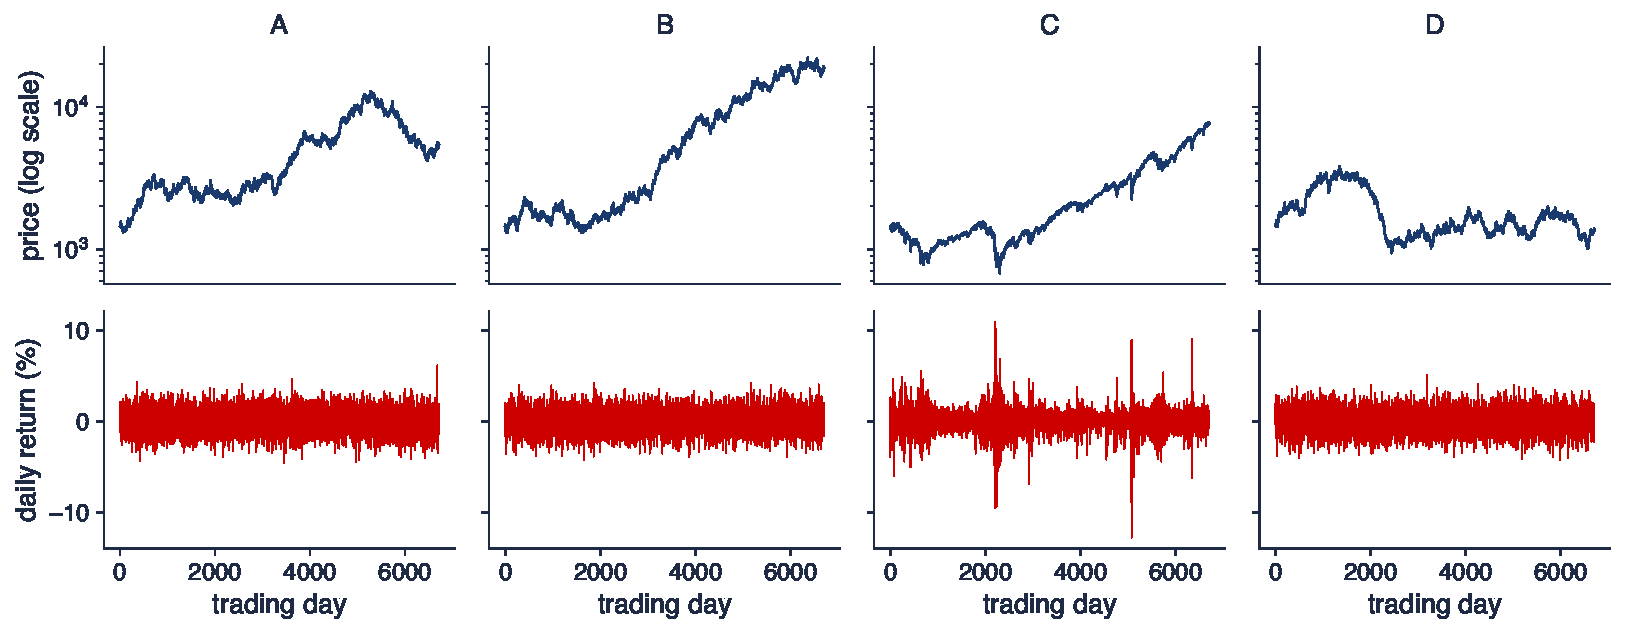
\includegraphics[width=0.97\textwidth,height=0.56\textheight,keepaspectratio]{sfm_ch4_spot_the_real.pdf}
\end{center}
\vspace{-0.25cm}
\begin{itemize}
    \item O coloană este S\&P 500, 2000--2026; trei sînt traiectorii GBM (randamente Normale i.i.d.) cu aceeași medie și volatilitate
    \item \textbf{Ce credeți?} Care coloană este reală, doar după prețuri?
    \item \textbf{Ce credeți?} Care coloană este reală, după randamente?
\end{itemize}
\sfmquantlet{Ch_04}{SFM_ch4_processes}
\end{frame}

\begin{frame}{Răspuns: coloana C}
\itemsize{\small}
\begin{itemize}
    \item \textbf{Răspuns}: coloana C este S\&P 500
    \item Prețurile: greu de spus; mersurile aleatoare cu tendință produc și ele avînturi și căderi lungi
    \begin{itemize}
        \item de aceea \refBachelier{} și \refOsborne{} au modelat prețurile ca mers aleator
    \end{itemize}
    \item Randamentele: diferența este evidentă; seria reală are ani liniștiți și episoade violente grupate (2008, 2020)
    \begin{itemize}
        \item exces de boltire 10{,}7 față de cel mult 0{,}02 în simulări; $\text{Corr}(r_t^2, r_{t-1}^2) = 0{,}31$ față de cel mult 0{,}006
        \item cea mai mare mișcare zilnică în valoare absolută 12{,}8\% față de 6{,}2\%
    \end{itemize}
    \item Lecția: un model poate reproduce traiectoria prețului și totuși să greșească în privința riscului
\end{itemize}
\end{frame}

\begin{frame}{Recapitulare: procese în timp discret}
\itemsize{\small}
\begin{itemize}
    \item Zgomot alb: necorelat; zgomot i.i.d.: independent; diferență de martingal: media imprevizibilă
    \item Mers aleator: șocuri permanente, varianța $t\sigma^2$; AR(1) cu $|\phi| < 1$: șocurile se sting în ritmul $\phi^h$
    \item Prețurile arată ca mersuri aleatoare; randamentele nu sînt i.i.d.
\end{itemize}
\end{frame}


%=============================================================================
\section{Procesul Wiener și mișcarea browniană geometrică}
%=============================================================================

\begin{frame}{De la polen la prețuri: mișcarea browniană}
\itemsize{\footnotesize}
\begin{columns}[T]
\begin{column}{0.60\textwidth}
\begin{itemize}
    \item 1827: botanistul Robert Brown observă mișcarea neregulată a particulelor de polen în apă
    \item 1900: Louis Bachelier modelează piața obligațiunilor de la Paris cu aceeași mișcare, cu cinci ani înaintea lui Einstein \refBachelier
    \item 1905: Albert Einstein o explică prin ciocniri moleculare \refEinstein
    \item 1923: Norbert Wiener construiește obiectul matematic riguros \refWiener
    \item 1959: \refOsborne{} o aplică prețurilor logaritmice: mișcarea browniană geometrică
\end{itemize}
\end{column}
\begin{column}{0.36\textwidth}
\begin{center}
\centering
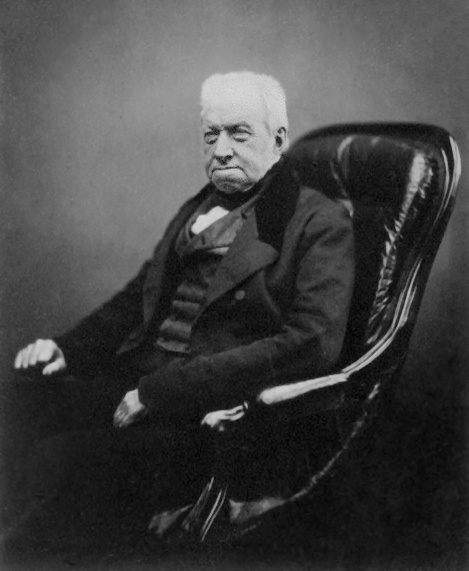
\includegraphics[height=0.20\textheight]{ch4_brown_1855.jpg}\\[1mm]
\imgcap{Robert Brown (1773--1858)}
\imgcredit{https://commons.wikimedia.org/wiki/File:Robert_Brown_(botanist).jpg}{Foto: Maull \& Polyblank (1855); domeniu public; Wikimedia Commons}\\[2mm]
\centering

\includegraphics[height=0.20\textheight]{ch0_bachelier.jpg}\\[1mm]
\imgcap{Louis Bachelier (1870--1946)}
\imgcredit{https://commons.wikimedia.org/wiki/File:LouisBachelier.jpg}{Foto: autor necunoscut; domeniu public; Wikimedia Commons}
\end{center}
\end{column}
\end{columns}
\end{frame}

\begin{frame}{Procesul Wiener}
\itemsize{\footnotesize}
\begin{columns}[T]
\begin{column}{0.64\textwidth}
\begin{itemize}
    \item $\{W(t), t \ge 0\}$ este un \textbf{proces Wiener} (mișcare browniană standard) dacă
    \begin{itemize}
        \item $W(0) = 0$
        \item creșterile pe intervale disjuncte sînt independente
        \item $W(t) - W(s) \sim N(0, t - s)$ pentru $s < t$: varianța este egală cu timpul scurs
        \item traiectoriile sînt continue
    \end{itemize}
    \item Limita mersului aleator scalat $W_n(t) = (\varepsilon_1 + \dots + \varepsilon_{\lfloor nt\rfloor})/\sqrt{n}$ (Donsker)
    \begin{itemize}
        \item $\varepsilon_i = \pm 1$, fiecare cu probabilitatea $1/2$; $n$ pași pe unitatea de timp
        \item $\lfloor nt\rfloor$: numărul de pași pînă la momentul $t$ (partea întreagă); împărțirea la $\sqrt{n}$ menține varianța egală cu $t$
    \end{itemize}
    \item Manual: \refFHH, cap.~5
\end{itemize}
\end{column}
\begin{column}{0.32\textwidth}
\centering
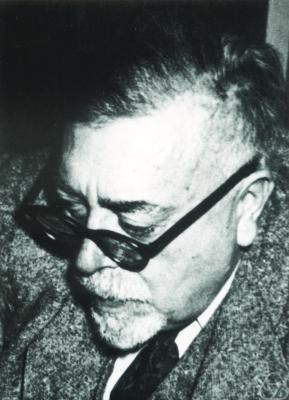
\includegraphics[height=0.50\textheight]{ch4_wiener.jpg}\\[1mm]
\imgcap{Norbert Wiener (1894--1964)}
\imgcredit{https://commons.wikimedia.org/wiki/File:Norbert_wiener.jpg}{Foto: Konrad Jacobs; CC BY-SA 2.0 DE; Wikimedia Commons}
\end{column}
\end{columns}
\end{frame}

\begin{frame}{De la mersul aleator la procesul Wiener (SFEWienerProcess)}
\itemsize{\footnotesize}
\begin{center}
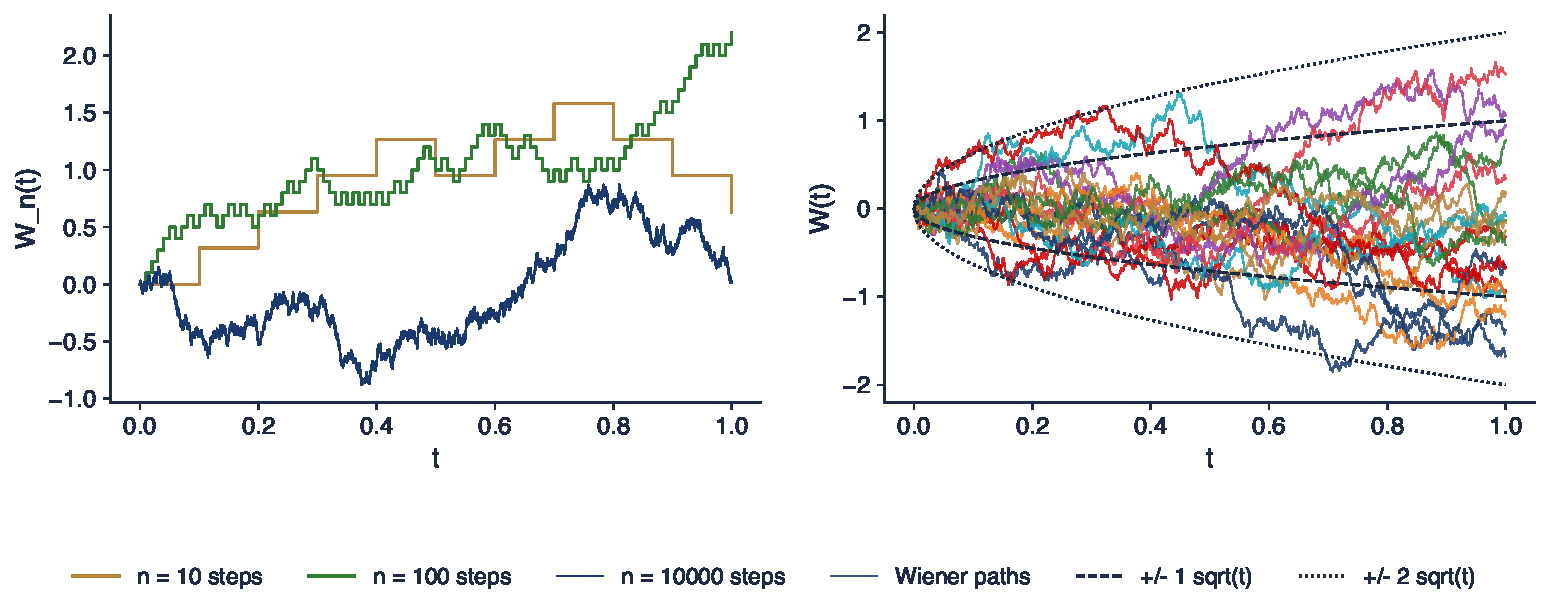
\includegraphics[width=0.97\textwidth,height=0.50\textheight,keepaspectratio]{sfm_ch4_wiener.pdf}
\end{center}
\vspace{-0.25cm}
\begin{itemize}
    \item Stînga: mersuri aleatoare scalate cu 10, 100 și 10\,000 de pași; treptele dispar, caracterul aleator rămîne
    \item Dreapta: 20 de traiectorii Wiener; $\text{Var}(W(t)) = t$, deci dispersia crește ca $\pm\sqrt{t}$
    \begin{itemize}
        \item $\text{Var}(W(1))$ simulată $= 1{,}006$; 68{,}2\% din valorile $W(1)$ în $\pm 1$ (teoretic 68{,}3\%)
    \end{itemize}
\end{itemize}
\sfmquantlet{Ch_04}{SFM_ch4_wiener_gbm}
\end{frame}

\begin{frame}{Proprietăți neobișnuite ale traiectoriilor Wiener}
\itemsize{\footnotesize}
\begin{itemize}
    \item Continue peste tot, nicăieri derivabile
    \begin{itemize}
        \item panta $(W(t + h) - W(t))/h \sim N(0, 1/h)$ are varianța $1/h$, care crește nelimitat cînd $h \to 0$
    \end{itemize}
    \item \textbf{Variația pătratică}: $\sum_k (W(t_{k+1}) - W(t_k))^2 \to t$ pe o grilă tot mai fină
    \begin{itemize}
        \item $0 = t_0 < t_1 < \dots < t$: grila; suma pătratelor creșterilor tinde către timpul scurs $t$
        \item 1000 de pași pe $[0, 1]$: media 0{,}999, abaterea standard 0{,}045 pe 10\,000 de traiectorii
        \item motivul pentru care $(dW)^2 = dt$ în calculul It\^o și pentru care varianța realizată măsoară volatilitatea (\sfmchlink{https://danpele.github.io/SFM/RO/Cursuri/capitol8_estimatori_volatilitate.pdf}{Capitolul 8})
    \end{itemize}
    \item $\text{Cov}(W(s), W(t)) = \min(s, t)$: $\text{Cov}(W(0{,}5), W(1))$ simulată $= 0{,}496$
    \item $W$ este un martingal; la fel și $W(t)^2 - t$
\end{itemize}
\end{frame}

\begin{frame}{Mișcarea browniană geometrică}
\itemsize{\footnotesize}
\begin{itemize}
    \item \textbf{GBM} (geometric Brownian motion, mișcarea browniană geometrică): $dS_t = \mu S_t\,dt + \sigma S_t\,dW_t$
    \begin{itemize}
        \item $dS_t$: variația prețului pe un interval foarte scurt $dt$
        \item $dW_t$: creșterea procesului Wiener pe intervalul $dt$, cu distribuția $N(0, dt)$
        \item variația relativă $dS/S$ are tendința (drift-ul) $\mu$ și volatilitatea $\sigma$, ambele anuale
    \end{itemize}
    \item Soluția: $S_t = S_0\exp\big((\mu - \sigma^2/2)t + \sigma W_t\big)$
    \begin{itemize}
        \item $\ln(S_t/S_0) \sim N\big((\mu - \sigma^2/2)t, \sigma^2 t\big)$
        \item prețuri lognormale, randamente logaritmice Normale i.i.d.
    \end{itemize}
    \item Modelul din spatele formulei \refBS{} (\sfmchlink{https://danpele.github.io/SFM/RO/Cursuri/capitol6_selectia_modelului_managementul_riscului.pdf}{capitolul 6} din manual)
\end{itemize}
\end{frame}

\begin{frame}{GBM: media, mediana și simularea}
\itemsize{\small}
\begin{itemize}
    \item Media $E[S_t] = S_0e^{\mu t}$; mediana $S_0e^{(\mu - \sigma^2/2)t}$
    \begin{itemize}
        \item mediana este mai mică: jumătate din traiectorii se termină sub $S_0e^{(\mu - \sigma^2/2)t}$
        \item diferența, $\sigma^2/2$ pe an în termeni logaritmici, este volatility drag
    \end{itemize}
    \item Simulare exactă pe o grilă: $S_{t + \Delta t} = S_t\exp\big((\mu - \sigma^2/2)\Delta t + \sigma\sqrt{\Delta t}\,Z\big)$
    \begin{itemize}
        \item $\Delta t$: pasul grilei, în ani; $Z \sim N(0, 1)$, o extragere nouă și independentă la fiecare pas
        \item exactă, pentru că fiecare creștere logaritmică este Normală, cu media și varianța corecte
    \end{itemize}
\end{itemize}
\end{frame}

\begin{frame}{GBM calibrat pe S\&P 500 (SFEsimGBM)}
\itemsize{\footnotesize}
\begin{center}
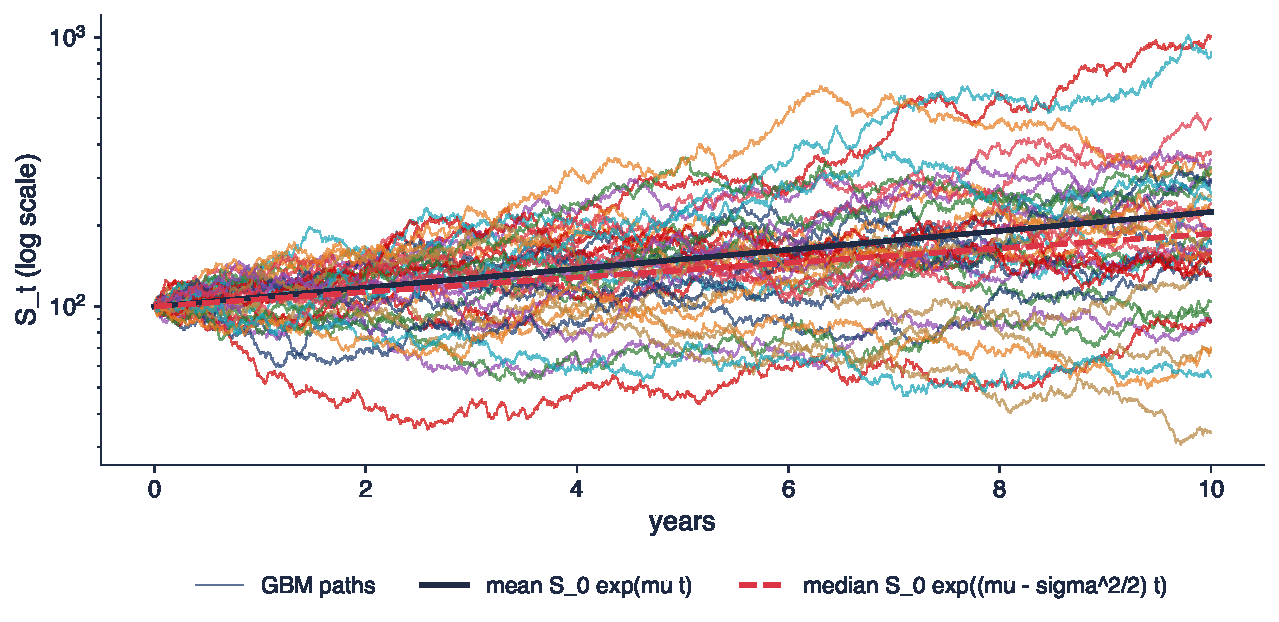
\includegraphics[width=0.97\textwidth,height=0.54\textheight,keepaspectratio]{sfm_ch4_gbm_paths.pdf}
\end{center}
\vspace{-0.25cm}
\begin{itemize}
    \item Calibrare, 2000--2026: $\sigma = 19{,}26\%$, tendința logaritmică $\mu - \sigma^2/2 = 6{,}23\%$, deci $\mu = 8{,}08\%$ pe an
    \item După $T = 10$ ani: media 224{,}4, mediana 186{,}4
    \begin{itemize}
        \item 62{,}0\% din traiectorii se termină sub medie; teoretic: $\Phi(\sigma\sqrt{T}/2) = 62{,}0\%$, cu $\Phi$ funcția de repartiție $N(0, 1)$
    \end{itemize}
    \item Probabilitatea unei pierderi după 10 ani: 15{,}3\%
\end{itemize}
\sfmquantlet{Ch_04}{SFM_ch4_wiener_gbm}
\end{frame}

\begin{frame}{Traiectorii reale în evantaiul GBM}
\itemsize{\scriptsize}
\begin{center}
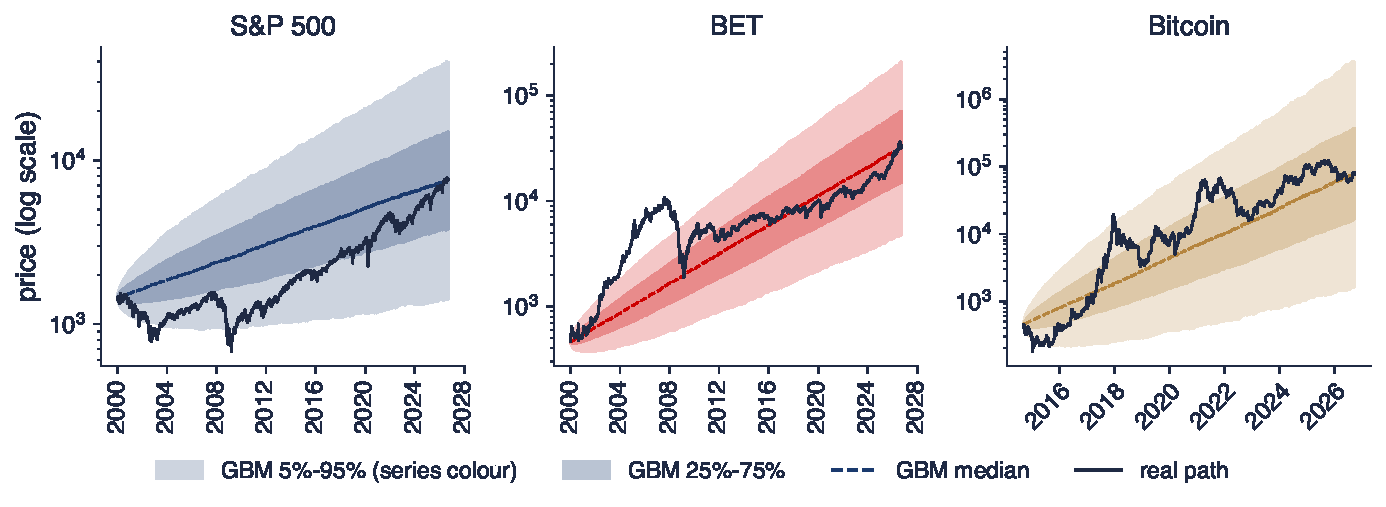
\includegraphics[width=0.97\textwidth,height=0.46\textheight,keepaspectratio]{sfm_ch4_gbm_fan.pdf}
\end{center}
\vspace{-0.25cm}
\begin{itemize}
    \item Fiecare evantai: 4000 de traiectorii GBM cu tendința și volatilitatea seriei respective, pornite din prima zi a seriei
    \item S\&P 500: traiectoria reală a coborît pînă la cuantila de 0{,}5\% pe 23 iulie 2002 și a încheiat perioada în jurul medianei
    \begin{itemize}
        \item în afara benzii de 90\% în 7\% din timp
    \end{itemize}
    \item BET: în afara benzii 24\% din timp
    \begin{itemize}
        \item avîntul din 2000--2007 și crahul din 2008 nu seamănă cu GBM
    \end{itemize}
    \item Bitcoin: cu $\sigma = 66{,}6\%$ pe an, evantaiul este foarte larg
    \begin{itemize}
        \item anualizată cu $A = 365$: activele cripto se tranzacționează în fiecare zi calendaristică ($A = 252$ pentru indici)
    \end{itemize}
\end{itemize}
\sfmquantlet{Ch_04}{SFM_ch4_wiener_gbm}
\end{frame}

\begin{frame}{Limitele modelului GBM}
\itemsize{\scriptsize}
\begin{center}
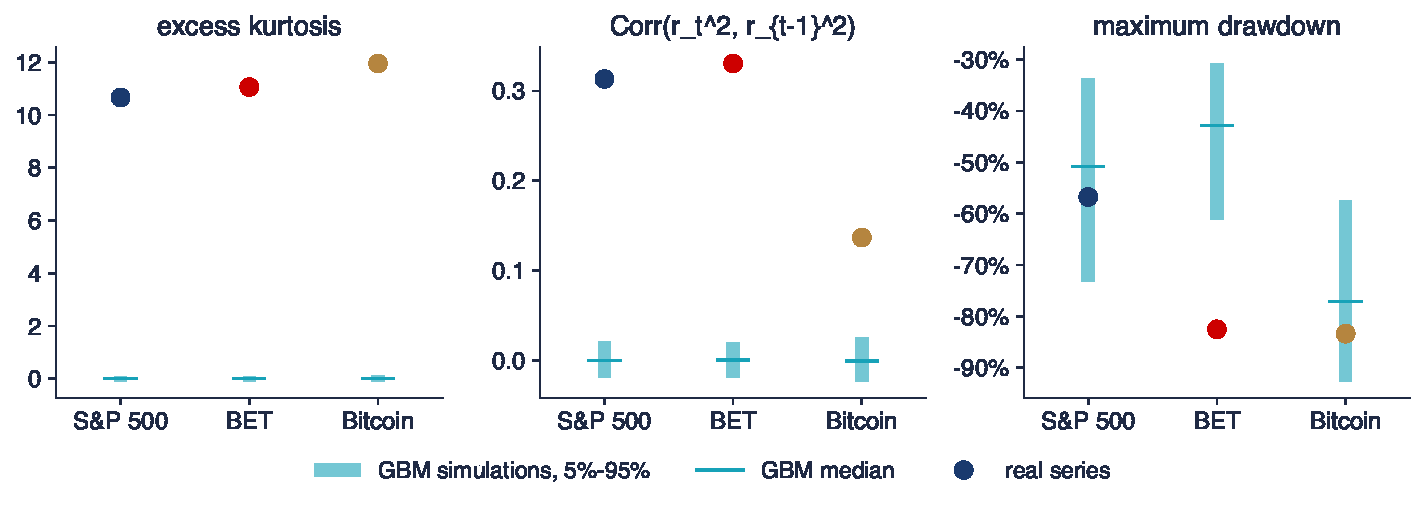
\includegraphics[width=0.97\textwidth,height=0.46\textheight,keepaspectratio]{sfm_ch4_gbm_check.pdf}
\end{center}
\vspace{-0.25cm}
\begin{itemize}
    \item Excesul de boltire: S\&P 500 10{,}7, BET 11{,}1, Bitcoin 12{,}0; 90\% din 300 de simulări GBM sînt în $[-0{,}10; 0{,}09]$
    \item Volatility clustering: $\text{Corr}(r_t^2, r_{t-1}^2) = 0{,}31$, $0{,}33$, $0{,}14$ față de cel mult $0{,}03$ în GBM
    \item Drawdown-ul maxim $\min_t \left(S_t/\max_{s \le t} S_s - 1\right)$: cea mai mare scădere față de un maxim anterior
    \begin{itemize}
        \item $-57\%$ la S\&P 500 este obișnuit în GBM; $-83\%$ la BET depășește 95\% din traiectorii (cuantila de 5\%: $-61\%$)
    \end{itemize}
    \item Zile de 4 sigma: 46 (S\&P 500) față de cel mult 1 în 95\% din traiectoriile GBM; criptomonedele au aceeași problemă \refPeleCrypto
\end{itemize}
\sfmquantlet{Ch_04}{SFM_ch4_wiener_gbm}
\end{frame}

\begin{frame}{Recapitulare: procesul Wiener și GBM}
\itemsize{\small}
\begin{itemize}
    \item Procesul Wiener: creșteri Normale independente, cu varianța egală cu timpul scurs
    \item GBM: prețuri lognormale, mediana sub medie, reperul evaluării opțiunilor
    \item Randamentele reale au cozi groase și volatility clustering, pe care GBM nu le poate genera
\end{itemize}
\end{frame}


%=============================================================================
\section{AI pentru descoperire științifică}
%=============================================================================

\begin{frame}{O întrebare deschisă: estimează GBM corect riscul de drawdown?}
\itemsize{\scriptsize}
\begin{center}
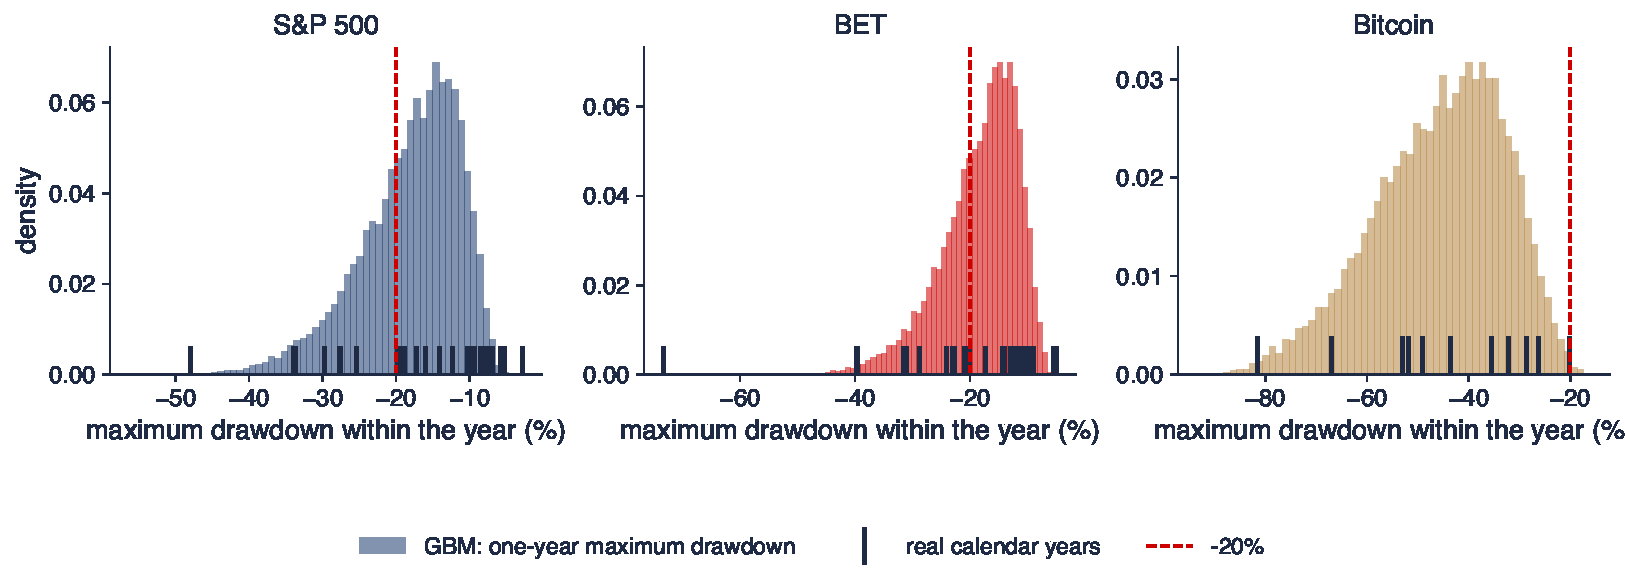
\includegraphics[width=0.97\textwidth,height=0.42\textheight,keepaspectratio]{sfm_ch4_drawdown_years.pdf}
\end{center}
\vspace{-0.25cm}
\begin{itemize}
    \item Drawdown: scăderea față de cel mai mare preț atins pînă atunci; aici, în cursul unui an calendaristic
    \begin{itemize}
        \item peste 20\%: S\&P 500 în 6 din 26 de ani (23\%), față de 34\% în GBM; BET 46\% față de 34\%
    \end{itemize}
    \item Peste 40\%: GBM prevede, în medie, 0{,}14 asemenea ani pentru S\&P 500 și 0{,}18 pentru BET
    \begin{itemize}
        \item fiecare indice a avut 1 (2008: $-48\%$ și $-73\%$)
    \end{itemize}
    \item Întrebare deschisă
    \begin{itemize}
        \item supraestimează GBM drawdown-urile moderate și le subestimează pe cele extreme pentru că anii calmi și cei de criză apar grupat?
    \end{itemize}
\end{itemize}
\sfmquantlet{Ch_04}{SFM_ch4_drawdown_open}
\end{frame}

\begin{frame}{Contribuția posibilă a AI}
\itemsize{\footnotesize}
\begin{itemize}
    \item \textbf{Literatura}: identificarea și rezumarea studiilor despre distribuția drawdown-urilor și legătura lor cu volatility clustering
    \item \textbf{Cod}: o primă versiune a simulărilor drawdown-urilor anuale în GBM, în bootstrap i.i.d. și într-un model GARCH
    \item \textbf{Design}: propunerea unui test care compară numărul observat de ani nefavorabili cu probabilitatea din model
    \item Exemplu de prompt
    \begin{itemize}
        \item \aiprompt{Write Python code that simulates 10,000 one-year paths of daily S\&P 500 returns under GBM and under an i.i.d.\ bootstrap of 2000-2026 returns, and returns the probability of a drawdown beyond 20\% and 40\% within the year.}
    \end{itemize}
\end{itemize}
\end{frame}

\begin{frame}{Verificări necesare}
\itemsize{\small}
\begin{itemize}
    \item Definițiile: drawdown-ul se calculează față de maximul atins pînă atunci în cursul anului, nu față de prima zi a anului
    \item Calibrarea: aceleași $\mu$ și $\sigma$, același număr de zile de tranzacționare pe an ca în date
    \item Inferența: 26 de ani reprezintă un eșantion mic; calculați un p-value binomial, nu doar proporții
    \item Mecanismul: bootstrap-ul i.i.d. păstrează cozile groase, dar elimină clustering-ul; diferența izolează efectul clustering-ului
    \item Referințele: fiecare lucrare citată trebuie să existe; verificați DOI-ul
\end{itemize}
\end{frame}

\begin{frame}{Idee de proiect}
\itemsize{\small}
\begin{itemize}
    \item \textbf{Întrebarea}: cît de mult greșește GBM probabilitatea unui an nefavorabil și de ce?
    \begin{itemize}
        \item date: S\&P 500, DAX, BET și Bitcoin din datele cursului
    \end{itemize}
    \item Pași
    \begin{itemize}
        \item calculați drawdown-ul maxim din fiecare an calendaristic
        \item simulați aceeași statistică în GBM, în bootstrap-ul i.i.d. și într-un model GARCH(1,1) (\sfmchlink{https://danpele.github.io/SFM/RO/Cursuri/capitol9_modele_arch_garch.pdf}{Capitolul 9})
        \item comparați ponderile peste 20\% și 40\% cu teste binomiale
    \end{itemize}
    \item Rezultat: un tabel, un grafic și un paragraf despre concluziile pe care datele le susțin și pe care nu le susțin
    \item Declarați orice folosire a AI și listați erorile AI pe care le-ați corectat \refWang
\end{itemize}
\end{frame}


%=============================================================================
\section{Rezumat}
%=============================================================================

\begin{frame}{Idei principale}
\itemsize{\small}
\begin{itemize}
    \item Distribuții: PMF, PDF, CDF și cuantile; VaR 1\% este minus o cuantilă
    \item Covarianța determină riscul portofoliului; randamentele necorelate nu sînt independente
    \item Varianța condiționată se schimbă cu știrile de ieri: punctul de plecare al GARCH
    \item Monte Carlo: transformarea inversă plus LLN; eroarea $\propto 1/\sqrt{N}$
    \item Arborele binomial $\to$ GBM; mers aleator, martingal, zgomot alb, AR(1)
    \item GBM reproduce aproximativ traiectoriile prețurilor, dar nu și cozile groase, volatility clustering și drawdown-urile extreme
\end{itemize}
\end{frame}

\begin{frame}{Formule de reținut}
\itemsize{\small}
\begin{center}
\footnotesize
\begin{tabular}{ll}
\toprule
\textbf{Mărimea} & \textbf{Formula} \\
\midrule
Varianța unei sume & $\text{Var}(aX + bY) = a^2\sigma_X^2 + b^2\sigma_Y^2 + 2ab\,\text{Cov}(X, Y)$ \\
Corelația & $\rho = \text{Cov}(X, Y)/(\sigma_X\sigma_Y)$ \\
Proprietatea turnului & $E[E[Y \mid X]] = E[Y]$ \\
Varianța totală & $\text{Var}(Y) = E[\text{Var}(Y \mid X)] + \text{Var}(E[Y \mid X])$ \\
Transformarea inversă & $X = F^{-1}(U)$, $U \sim U(0, 1)$ \\
Eroarea Monte Carlo & $\sqrt{p(1 - p)/N}$ \\
Mers aleator & $S_t = S_{t-1} + \mu + \varepsilon_t$, $\text{Var}(S_t) = t\sigma^2$ \\
AR(1) & $\text{Var}(X_t) = \sigma^2/(1 - \phi^2)$, $\rho(h) = \phi^h$ \\
GBM & $S_t = S_0\exp((\mu - \sigma^2/2)t + \sigma W_t)$, $E[S_t] = S_0e^{\mu t}$ \\
\bottomrule
\end{tabular}
\end{center}
\end{frame}

\begin{frame}{Autoevaluare}
\itemsize{\small}
\begin{itemize}
    \item \textbf{Întrebare}: $\sigma_1 = 2\%$, $\sigma_2 = 3\%$, $\rho = 0{,}5$; cît este volatilitatea portofoliului 50/50?
    \begin{itemize}
        \item \textbf{Răspuns}: $\sqrt{0{,}25 \times 4 + 0{,}25 \times 9 + 2 \times 0{,}25 \times 0{,}5 \times 2 \times 3} = \sqrt{4{,}75} = 2{,}18\%$
    \end{itemize}
    \item \textbf{Întrebare}: GBM cu $\mu = 8\%$, $\sigma = 20\%$, $S_0 = 100$; cît sînt media și mediana lui $S_1$?
    \begin{itemize}
        \item \textbf{Răspuns}: media $100e^{0{,}08} = 108{,}33$, mediana $100e^{0{,}06} = 106{,}18$
    \end{itemize}
    \item \textbf{Întrebare}: AR(1) cu $\phi = 0{,}8$ și $\sigma = 1$; cît este varianța lui?
    \begin{itemize}
        \item \textbf{Răspuns}: $1/(1 - 0{,}64) = 2{,}78$
    \end{itemize}
    \item Urmează: \sfmchlink{https://danpele.github.io/SFM/RO/Cursuri/capitol5_cozi_groase_evt.pdf}{Capitolul 5}, cozi groase și teoria valorilor extreme
\end{itemize}
\end{frame}


%=============================================================================
\section{Bibliografie}
%=============================================================================

\begin{frame}{Bibliografie (1/2)}
\itemsize{\tiny}
\begin{itemize}
    \item Bachelier, L. (1900). \href{https://doi.org/10.24033/asens.476}{Théorie de la spéculation}. \textit{Annales scientifiques de l'École Normale Supérieure}, 17, 21--86.
    \item Black, F., Scholes, M. (1973). \href{https://doi.org/10.1086/260062}{The pricing of options and corporate liabilities}. \textit{Journal of Political Economy}, 81(3), 637--654.
    \item Bollerslev, T. (1986). \href{https://doi.org/10.1016/0304-4076(86)90063-1}{Generalized autoregressive conditional heteroskedasticity}. \textit{Journal of Econometrics}, 31(3), 307--327.
    \item Borak, S., Härdle, W.K., López-Cabrera, B. (2013). \href{https://doi.org/10.1007/978-3-642-33929-5}{\textit{Statistics of Financial Markets: Exercises and Solutions}}, 2nd ed. Springer.
    \item Cont, R. (2001). \href{https://doi.org/10.1080/713665670}{Empirical properties of asset returns: stylized facts and statistical issues}. \textit{Quantitative Finance}, 1(2), 223--236.
    \item Cox, J.C., Ross, S.A., Rubinstein, M. (1979). \href{https://doi.org/10.1016/0304-405X(79)90015-1}{Option pricing: a simplified approach}. \textit{Journal of Financial Economics}, 7(3), 229--263.
    \item Einstein, A. (1905). \href{https://doi.org/10.1002/andp.19053220806}{Über die von der molekularkinetischen Theorie der Wärme geforderte Bewegung von in ruhenden Flüssigkeiten suspendierten Teilchen}. \textit{Annalen der Physik}, 322(8), 549--560.
    \item Engle, R.F. (1982). \href{https://doi.org/10.2307/1912773}{Autoregressive conditional heteroscedasticity with estimates of the variance of United Kingdom inflation}. \textit{Econometrica}, 50(4), 987--1007.
    \item Fama, E.F. (1970). \href{https://doi.org/10.2307/2325486}{Efficient capital markets: a review of theory and empirical work}. \textit{Journal of Finance}, 25(2), 383--417.
    \item Franke, J., Härdle, W.K., Hafner, C.M. (2019). \href{https://doi.org/10.1007/978-3-030-13751-9}{\textit{Statistics of Financial Markets: An Introduction}}, 5th ed. Springer.
\end{itemize}
\end{frame}

\begin{frame}{Bibliografie (2/2)}
\itemsize{\tiny}
\begin{itemize}
    \item Glasserman, P. (2003). \href{https://doi.org/10.1007/978-0-387-21617-1}{\textit{Monte Carlo Methods in Financial Engineering}}. Springer.
    \item Kolmogoroff, A. (1933). \href{https://doi.org/10.1007/978-3-642-49888-6}{\textit{Grundbegriffe der Wahrscheinlichkeitsrechnung}}. Springer, Berlin.
    \item Marsaglia, G. (1968). \href{https://doi.org/10.1073/pnas.61.1.25}{Random numbers fall mainly in the planes}. \textit{Proceedings of the National Academy of Sciences}, 61(1), 25--28.
    \item Matsumoto, M., Nishimura, T. (1998). \href{https://doi.org/10.1145/272991.272995}{Mersenne twister: a 623-dimensionally equidistributed uniform pseudo-random number generator}. \textit{ACM Transactions on Modeling and Computer Simulation}, 8(1), 3--30.
    \item Metropolis, N., Ulam, S. (1949). \href{https://doi.org/10.1080/01621459.1949.10483310}{The Monte Carlo method}. \textit{Journal of the American Statistical Association}, 44(247), 335--341.
    \item Osborne, M.F.M. (1959). \href{https://doi.org/10.1287/opre.7.2.145}{Brownian motion in the stock market}. \textit{Operations Research}, 7(2), 145--173.
    \item Pele, D.T., Wesselhöfft, N., Härdle, W.K., Kolossiatis, M., Yatracos, Y.G. (2023). \href{https://doi.org/10.1080/1351847X.2021.1960403}{Are cryptos becoming alternative assets?} \textit{European Journal of Finance}, 29(10), 1064--1105.
    \item Wang, H., Fu, T., Du, Y., Gao, W., et al. (2023). \href{https://doi.org/10.1038/s41586-023-06221-2}{Scientific discovery in the age of artificial intelligence}. \textit{Nature}, 620, 47--60.
    \item Wiener, N. (1923). \href{https://doi.org/10.1002/sapm192321131}{Differential-space}. \textit{Journal of Mathematics and Physics}, 2(1--4), 131--174.
\end{itemize}
\end{frame}

\end{document}
